\documentclass{article}
\usepackage{graphicx}

\title{APLIKASI APEX}
\author{nurulkamila1899 }
\date{November 2019}

\begin{document}

\maketitle

\section{Cara Membuat Aplikasi Builder dari File Exel ke Oracle Apex}
\begin{enumerate}
    \item Buka Oracle Apex, lalu masukkan workspace, username beserta password dan sign in
    \item Jika sudah masuk, klik App Builder
    \item Selanjutnya klik Creat
    \begin{center}
    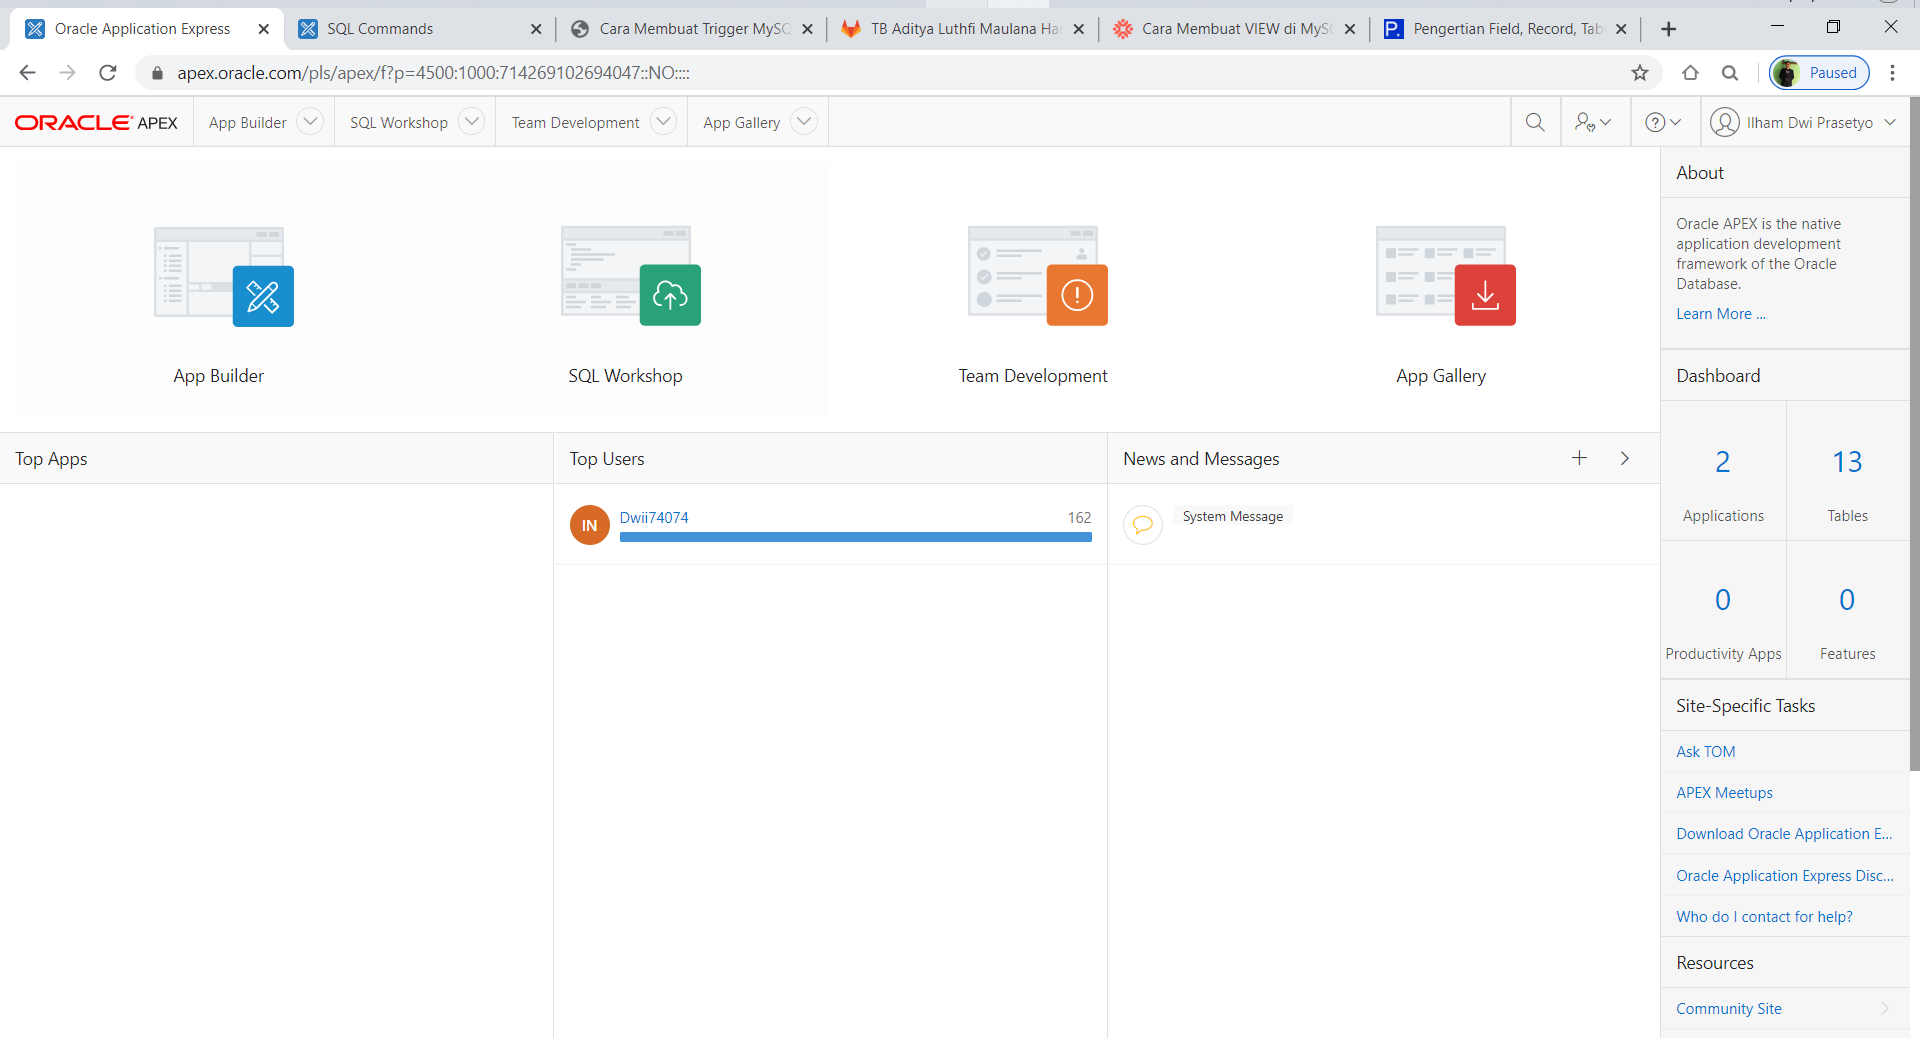
\includegraphics[width=.8\textwidth]{fifure/1.PNG}
    \end{center}
    \item Pada laman Creat an Application, pilih Form a File
     \begin{center}
    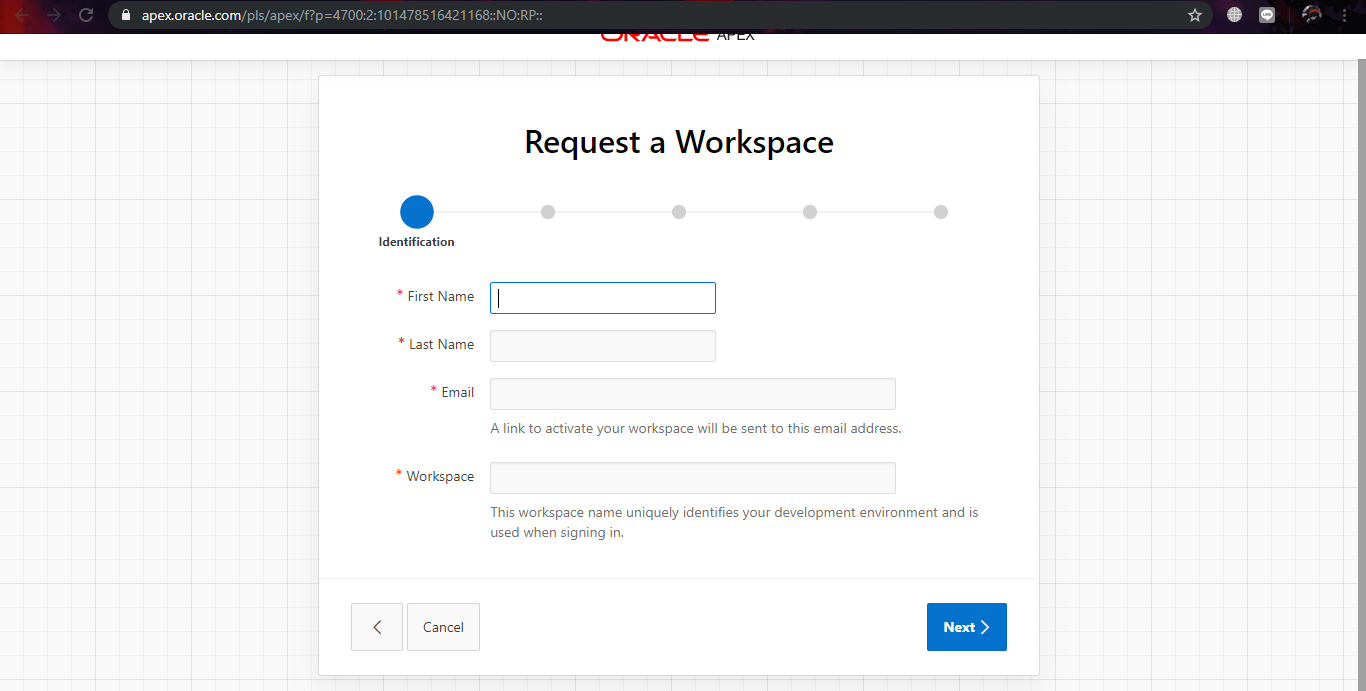
\includegraphics[width=.8\textwidth]{fifure/2.PNG}
    \end{center}
    \item Lalu, klik Choose File dan pilih file exel yang berisikan data , seperti contoh di bawah ini
    \begin{center}
    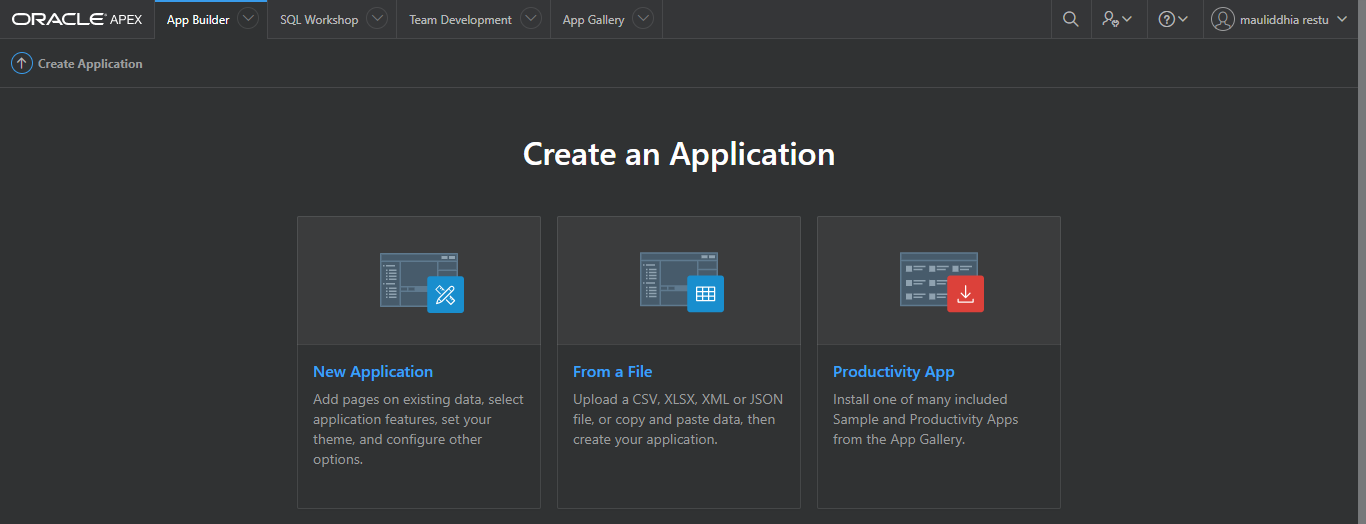
\includegraphics[width=.8\textwidth]{fifure/3.PNG}
    \end{center}
    \item Pada laman selanjutnya, silahkan masukkan nama Table sesuai yang kamu inginkan, perlu diketahui pada kolom error table name akan terisi otomatis. setelah itu klik Configure, lalu save change.
    \begin{center}
    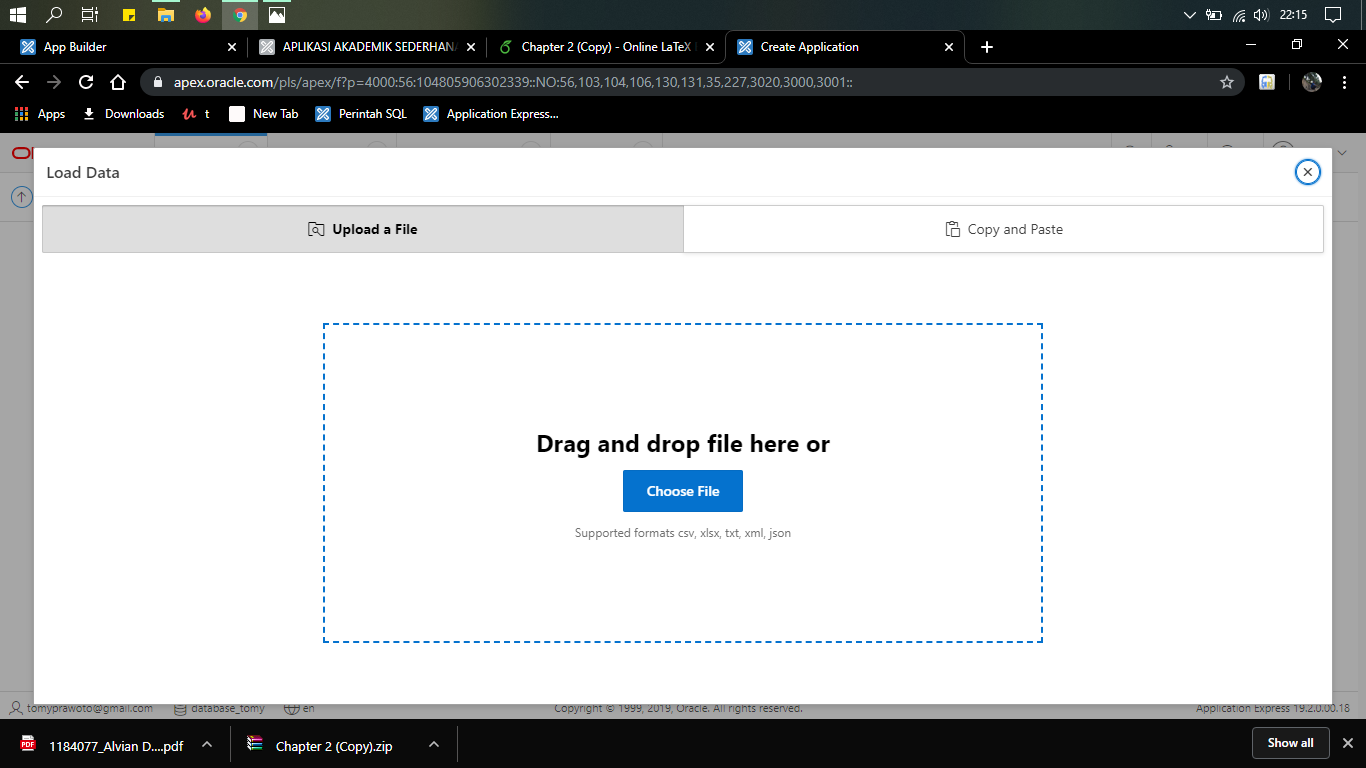
\includegraphics[width=.8\textwidth]{fifure/4.PNG}
    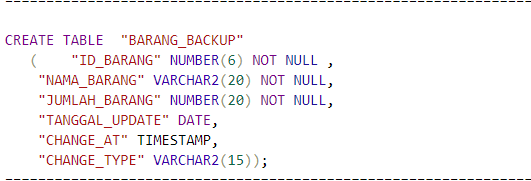
\includegraphics[width=.8\textwidth]{fifure/5.PNG}
    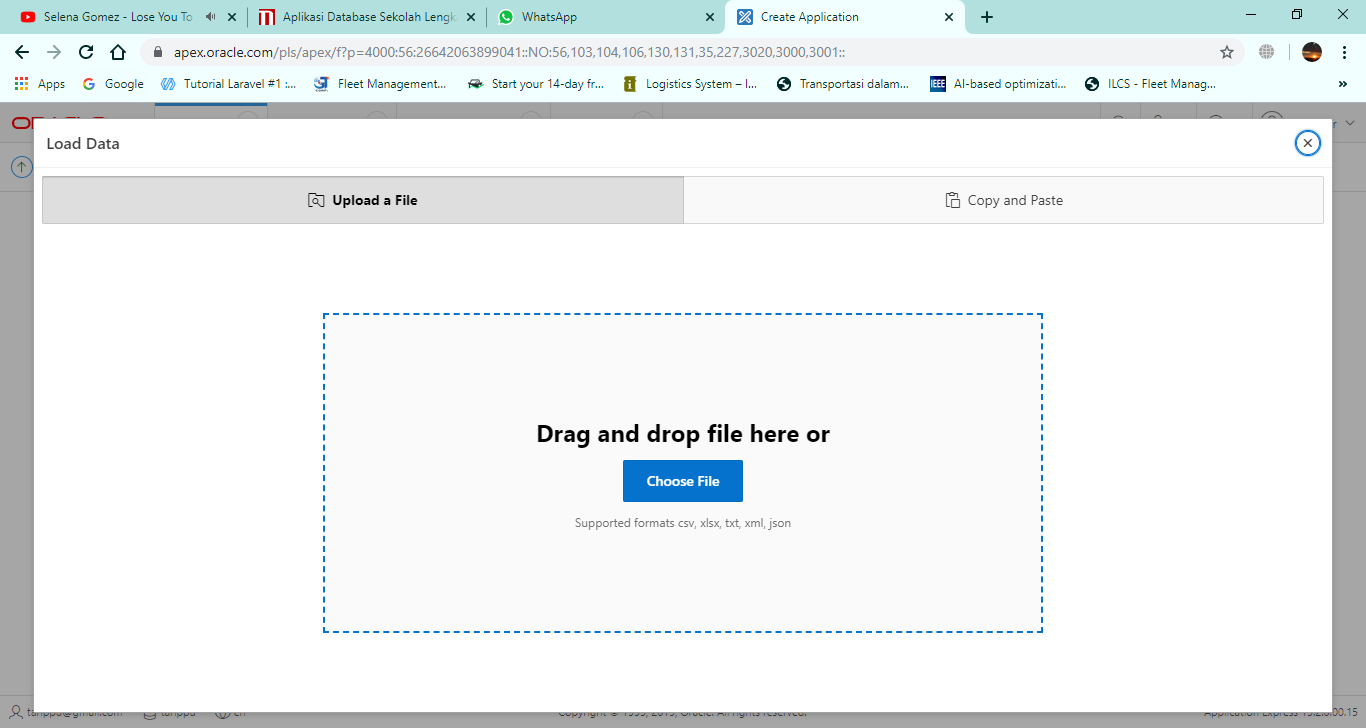
\includegraphics[width=.8\textwidth]{fifure/6.PNG}
    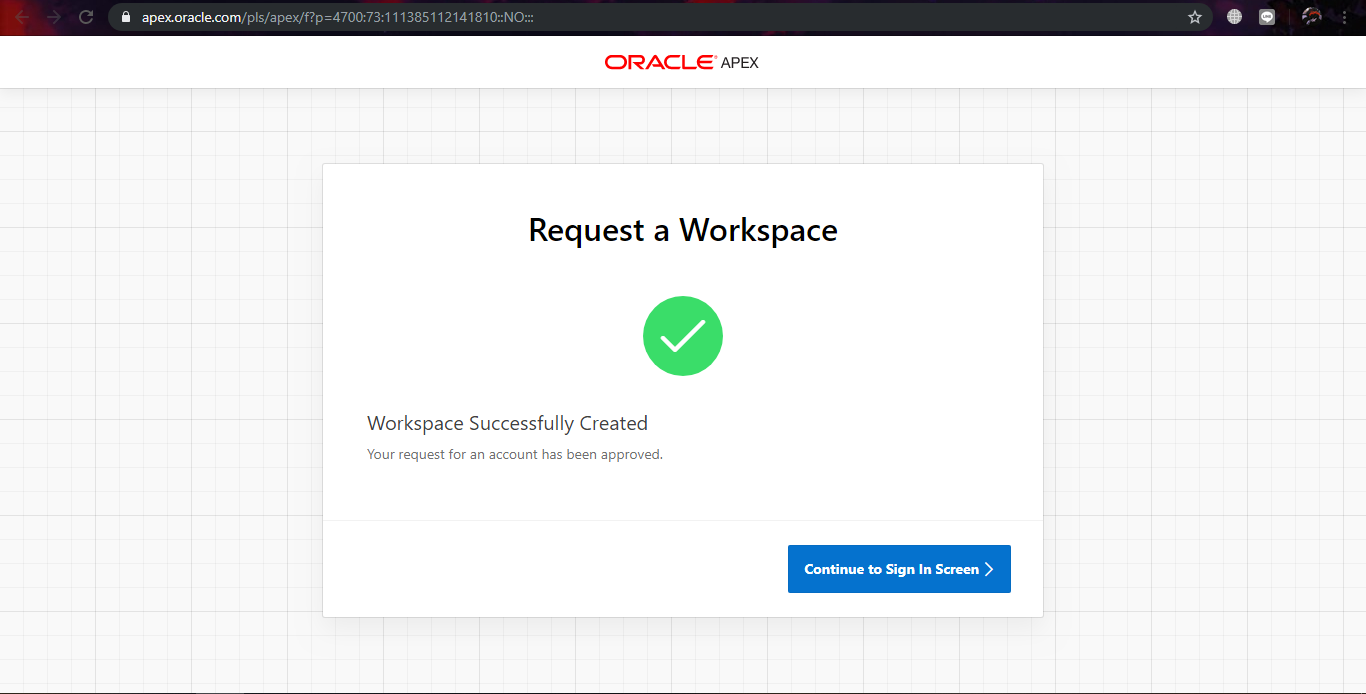
\includegraphics[width=.8\textwidth]{fifure/7.PNG}
    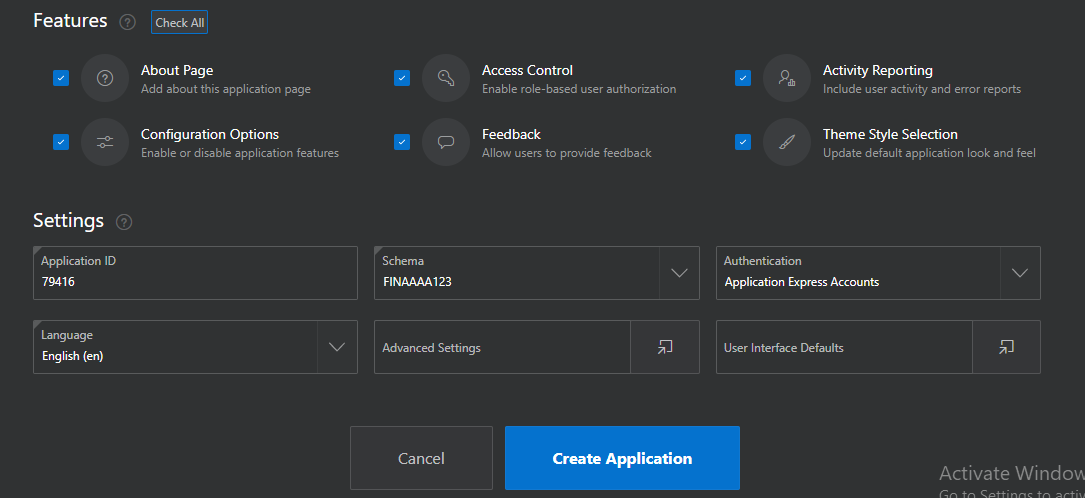
\includegraphics[width=.8\textwidth]{fifure/8.PNG}
    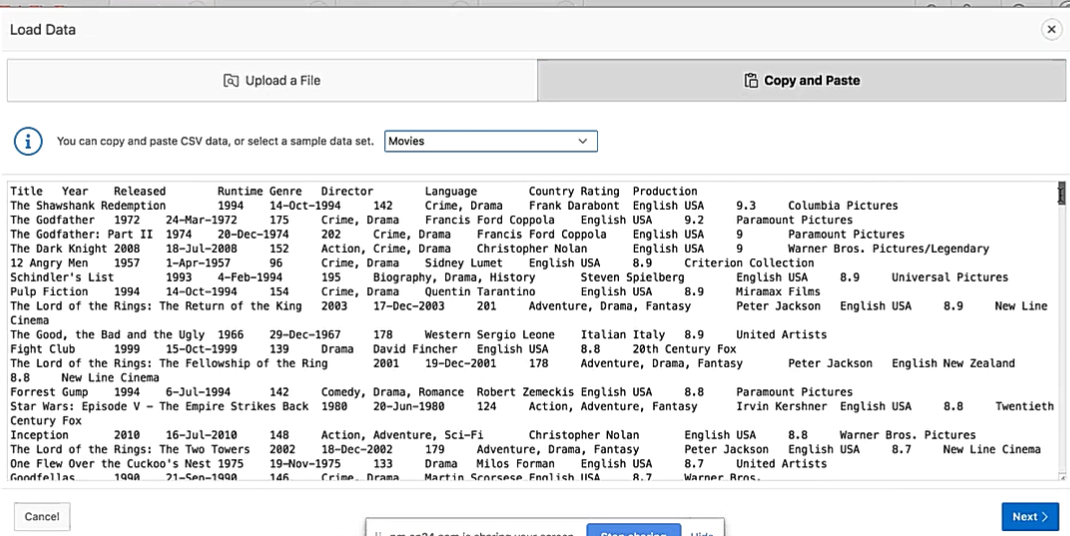
\includegraphics[width=.8\textwidth]{fifure/9.PNG}
    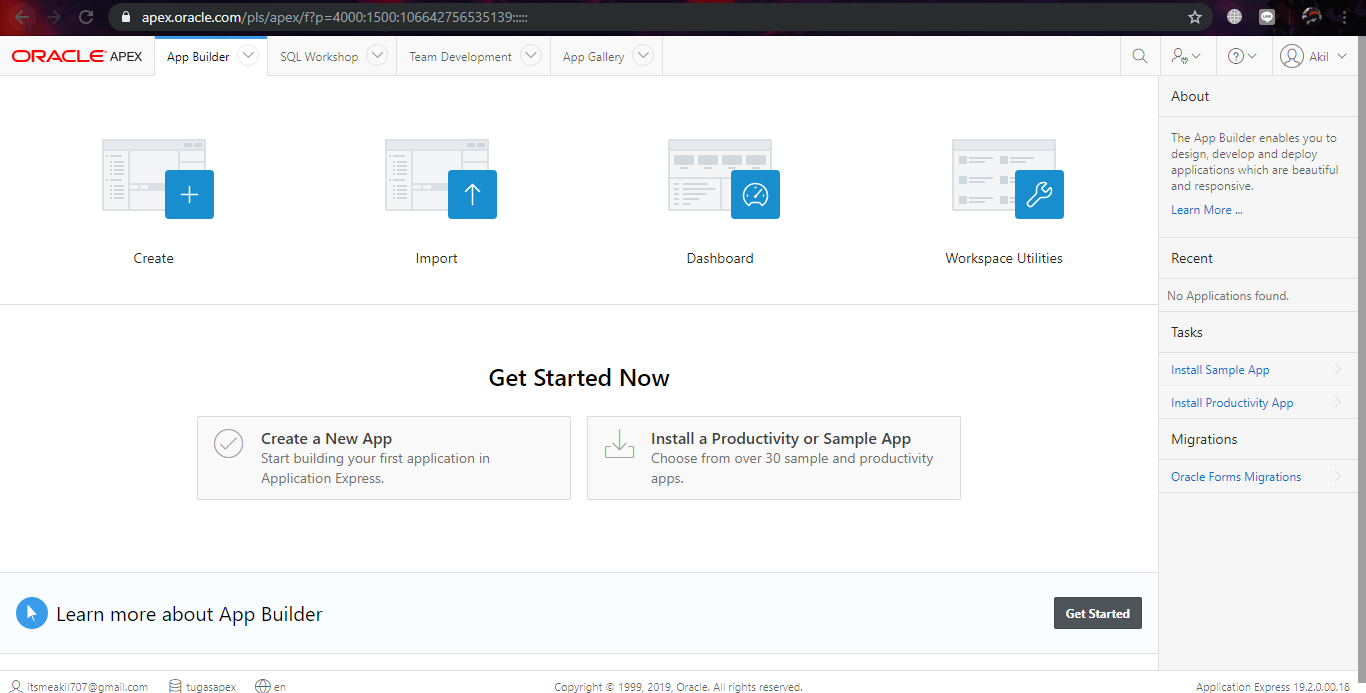
\includegraphics[width=.8\textwidth]{fifure/10.PNG}
    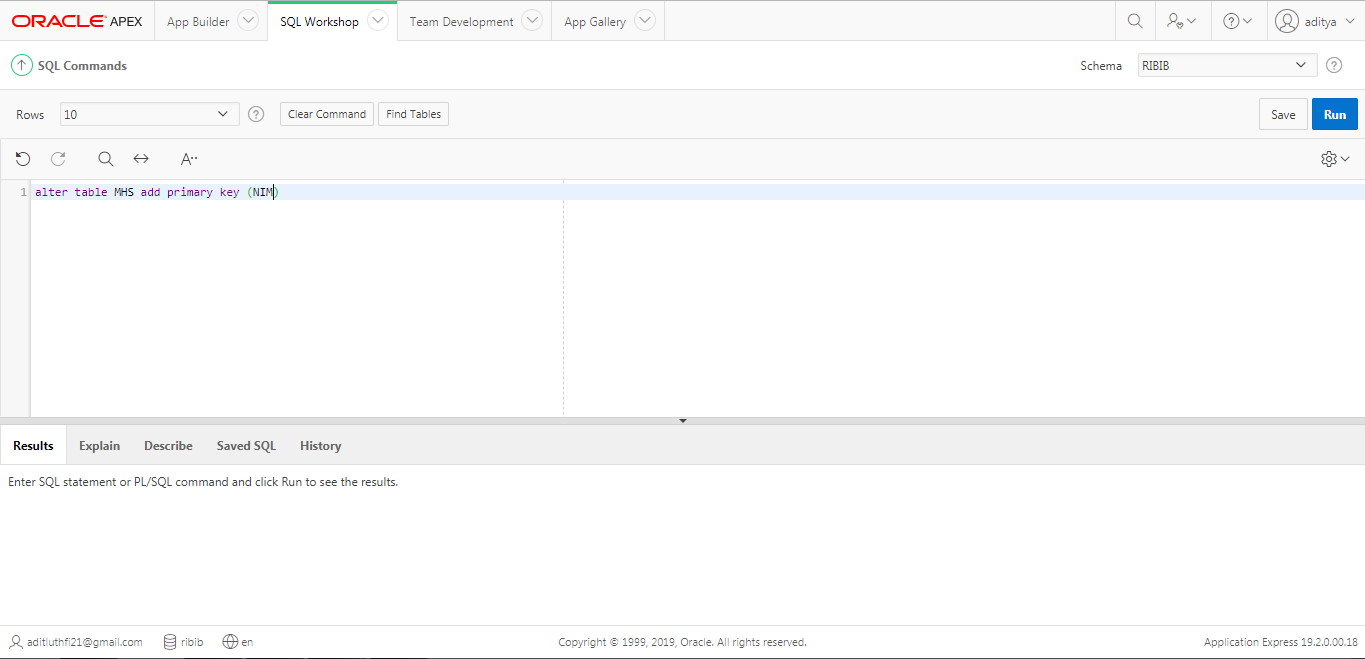
\includegraphics[width=.8\textwidth]{fifure/11.PNG}
    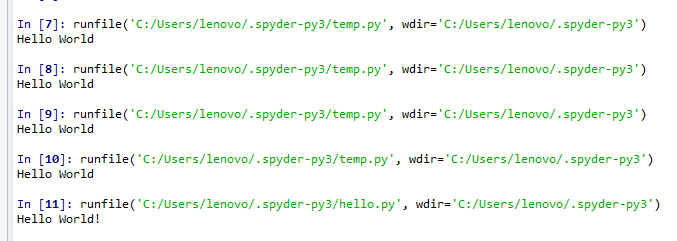
\includegraphics[width=.8\textwidth]{fifure/12.PNG}
    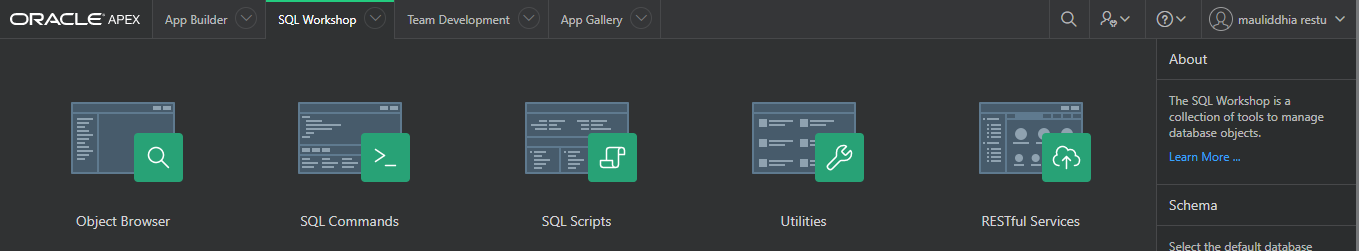
\includegraphics[width=.8\textwidth]{fifure/13.PNG}
    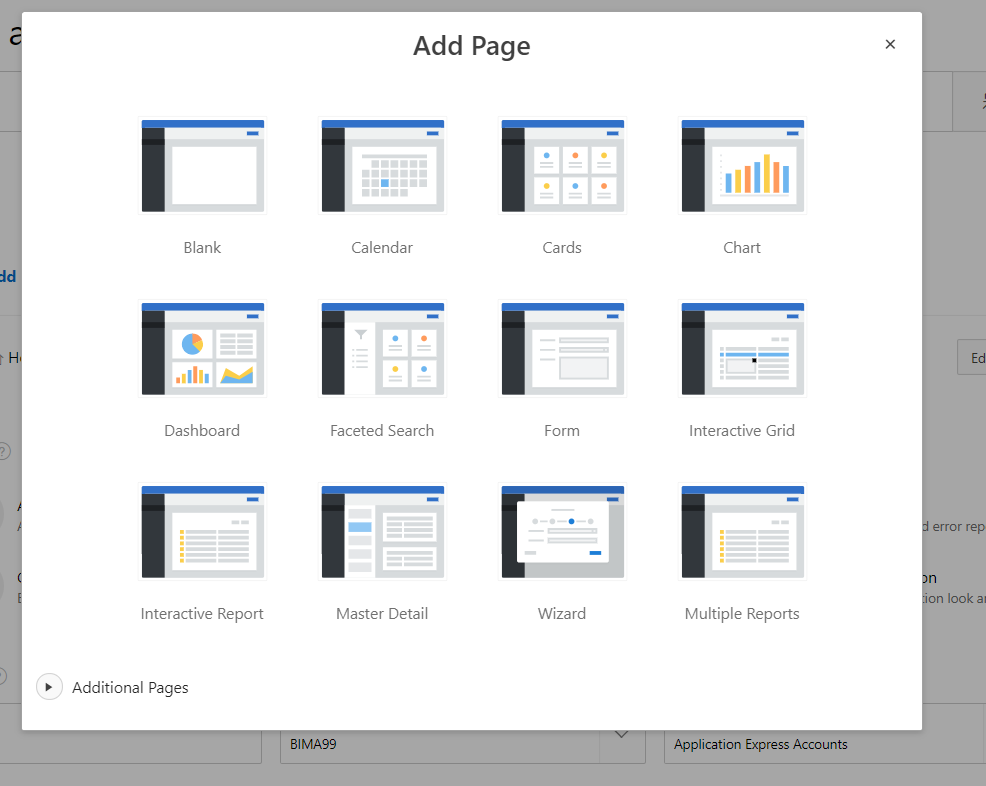
\includegraphics[width=.8\textwidth]{fifure/14.PNG}
    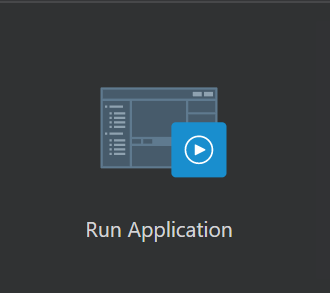
\includegraphics[width=.8\textwidth]{fifure/15.PNG}
    \end{center}
    \item Kita dapat melihat table kita pada SQL WorkShop
     \begin{center}
    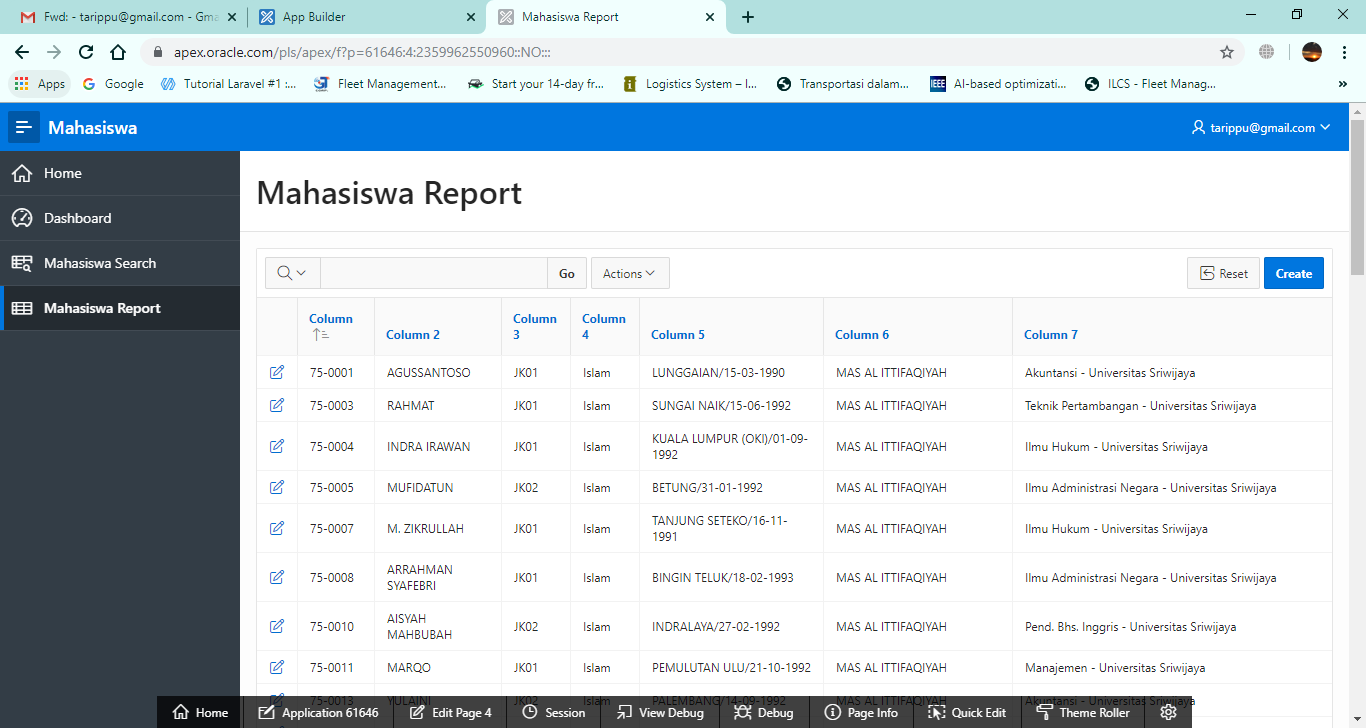
\includegraphics[width=.8\textwidth]{fifure/16.PNG}
    \end{center}
    \item Hilangkan kolom ID(number) pada setiap tabel
     \begin{center}
    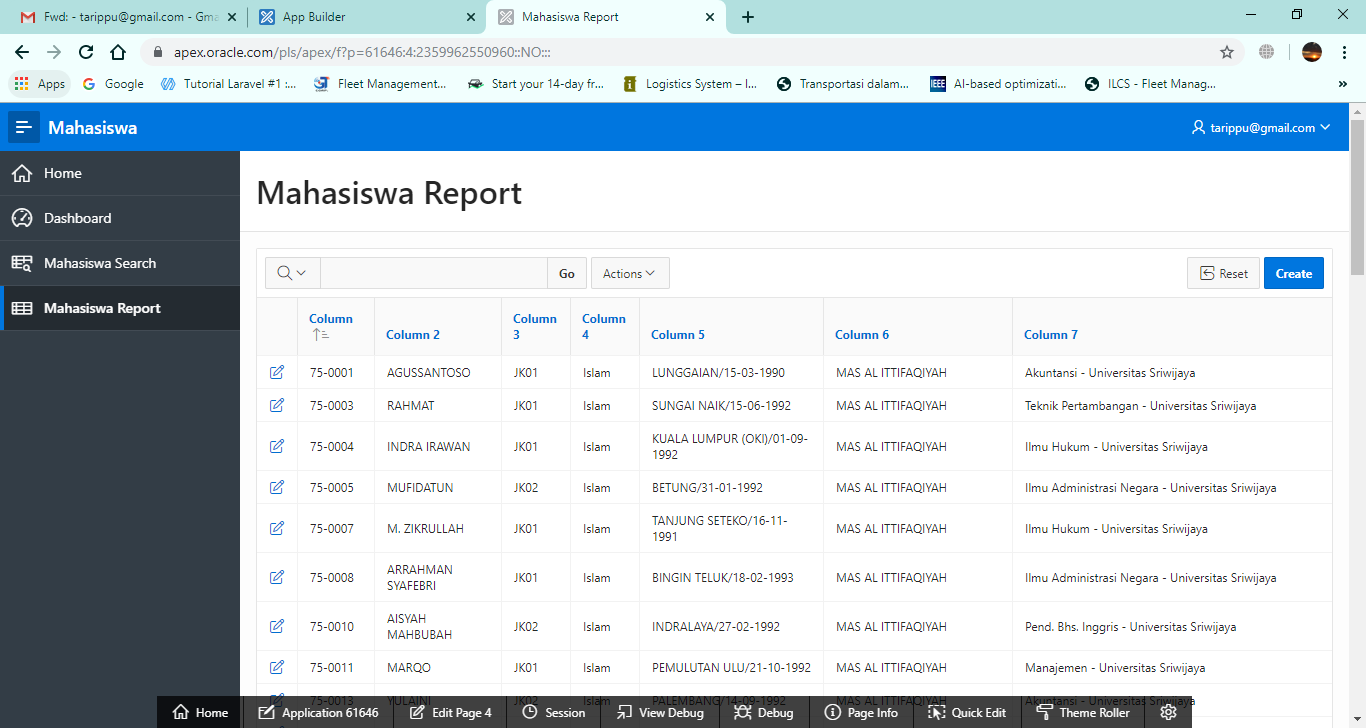
\includegraphics[width=.8\textwidth]{fifure/16.PNG}
    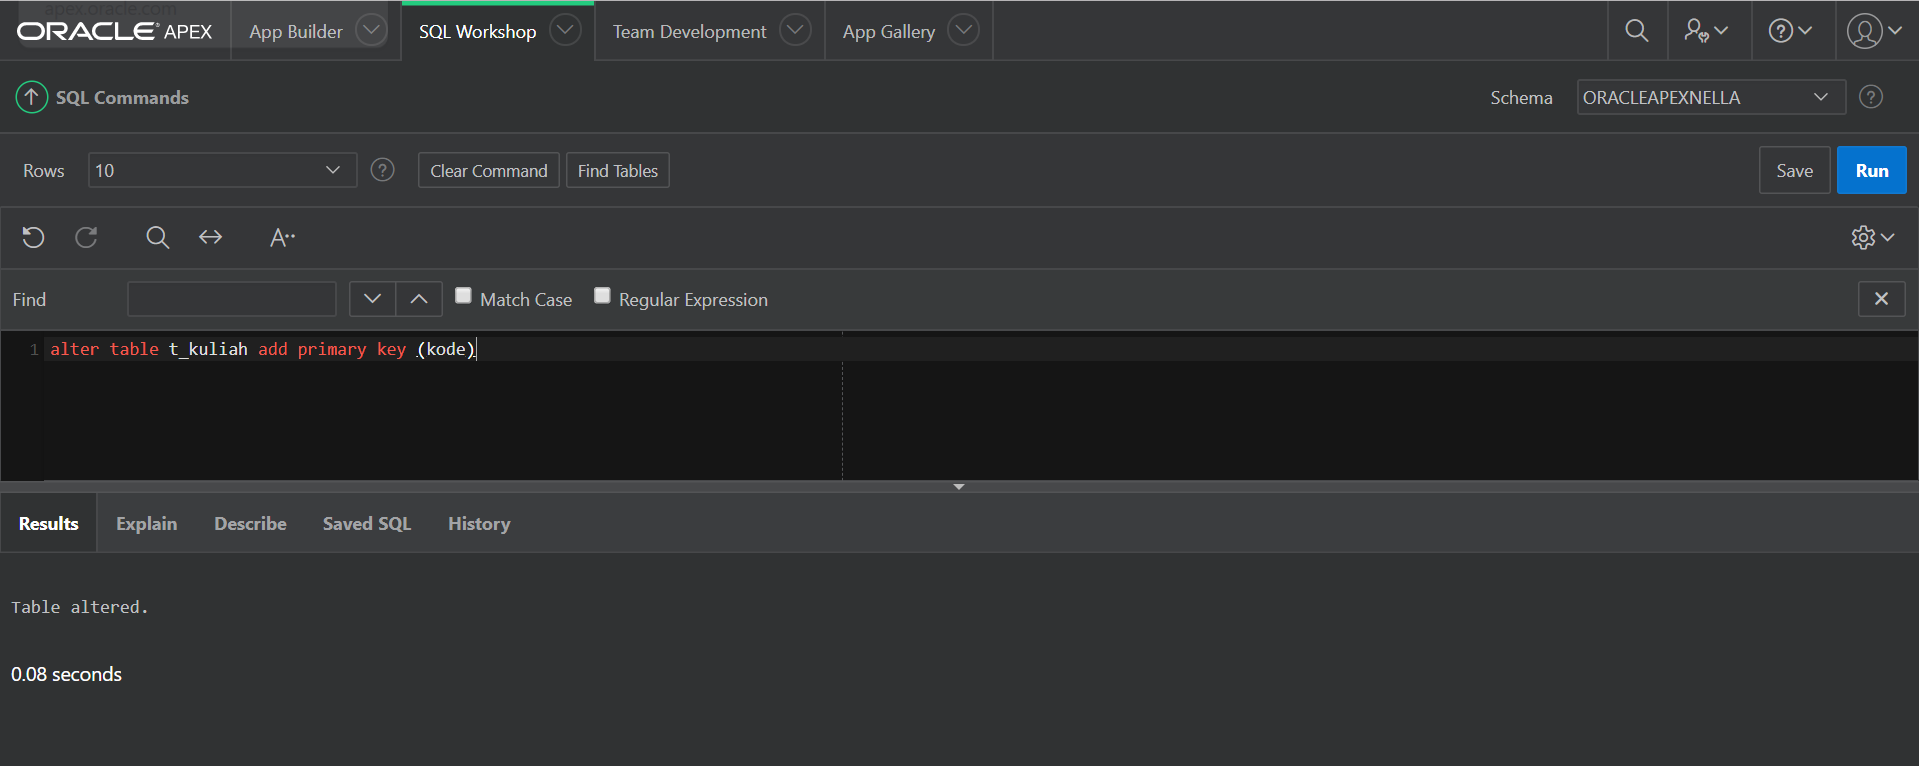
\includegraphics[width=.8\textwidth]{fifure/17.PNG}
    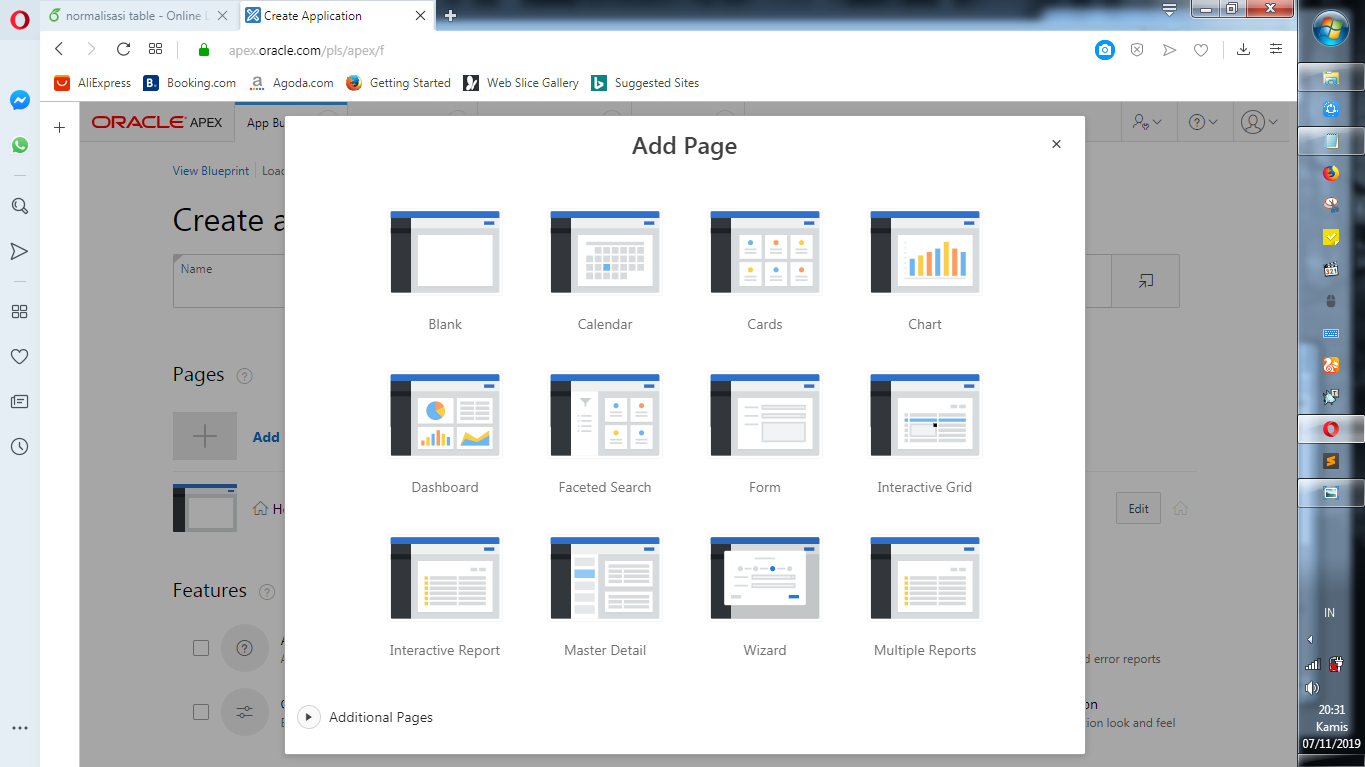
\includegraphics[width=.8\textwidth]{fifure/18.PNG}
    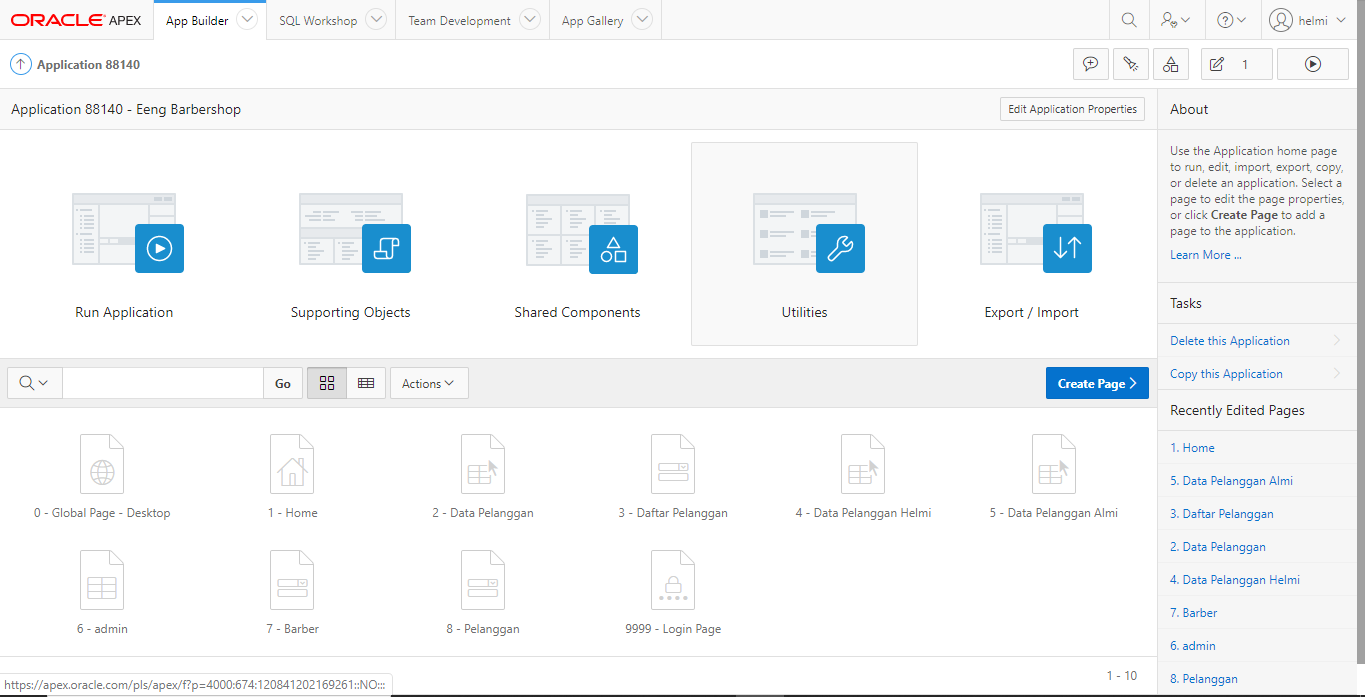
\includegraphics[width=.8\textwidth]{fifure/19.PNG}
    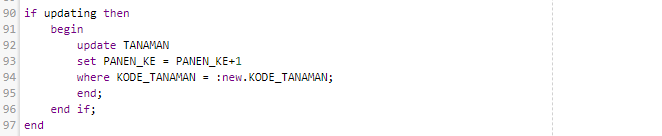
\includegraphics[width=.8\textwidth]{fifure/20.PNG}
    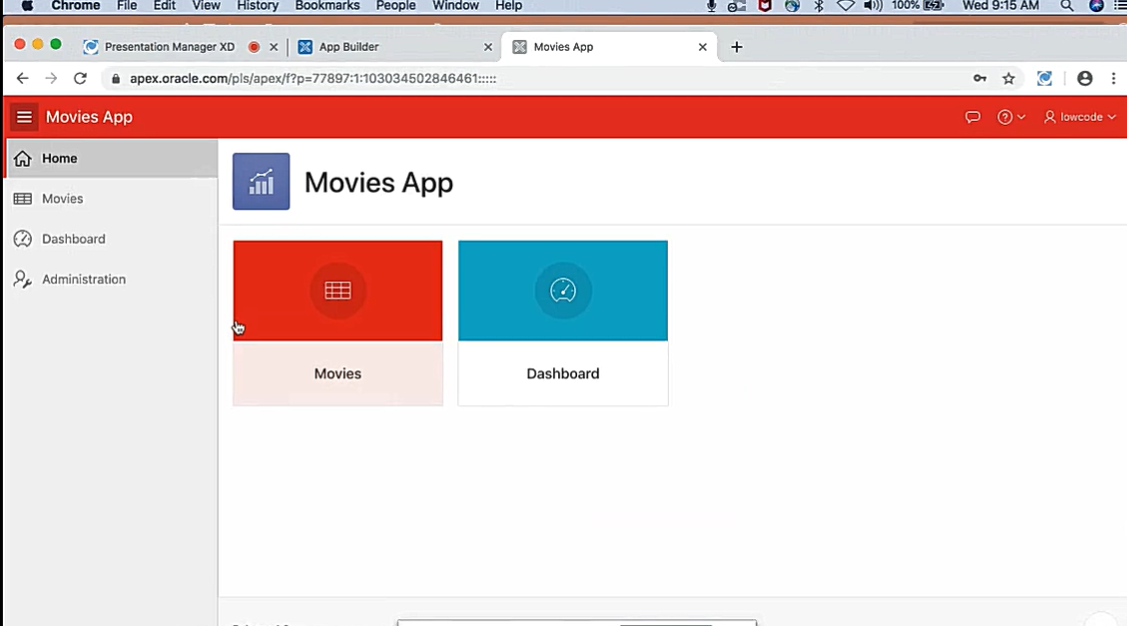
\includegraphics[width=.8\textwidth]{fifure/21.PNG}
    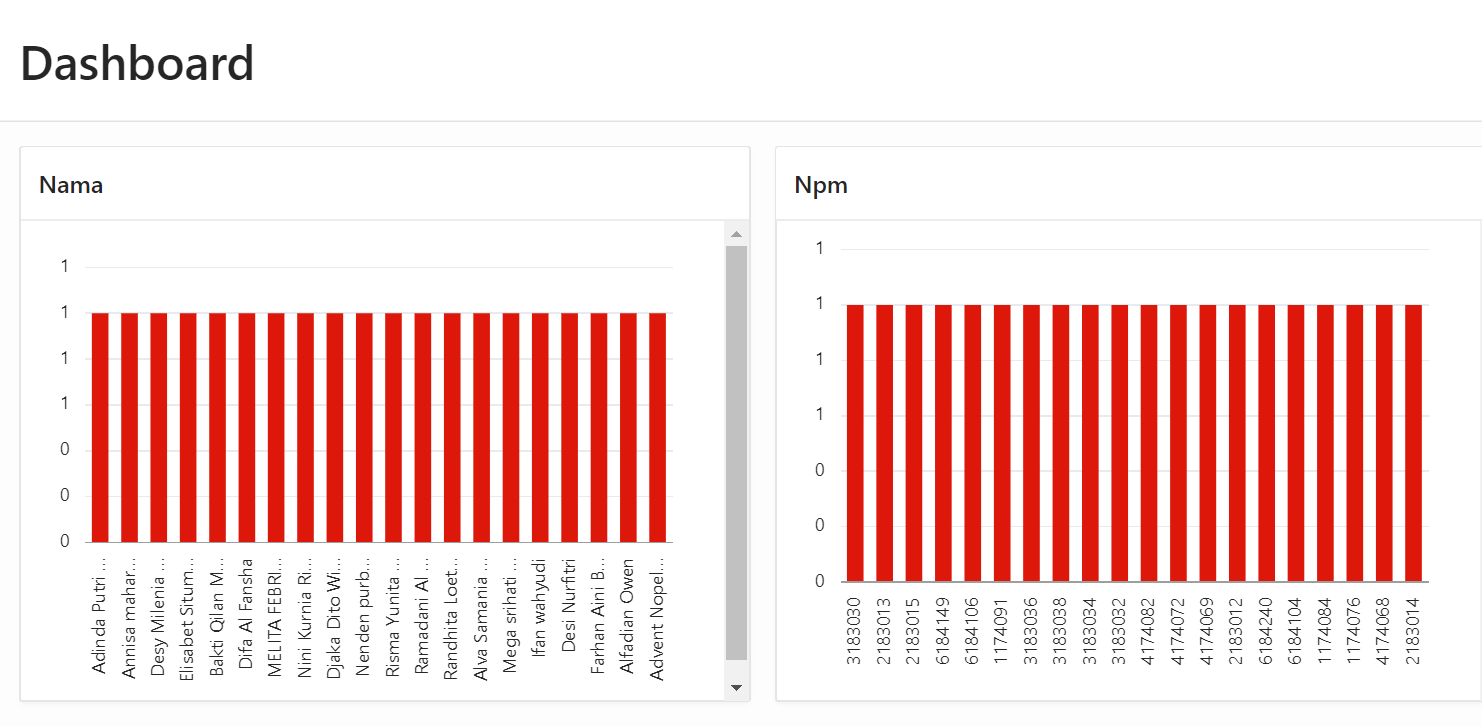
\includegraphics[width=.8\textwidth]{fifure/22.PNG}
    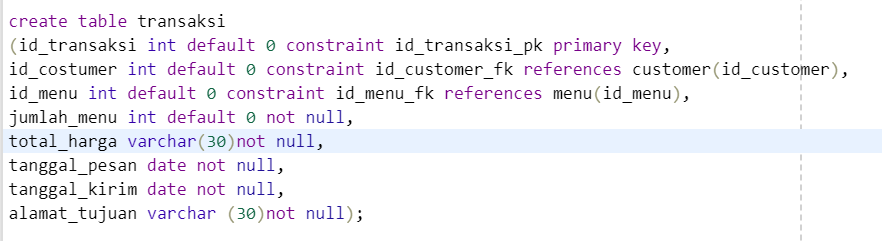
\includegraphics[width=.8\textwidth]{fifure/23.PNG}
    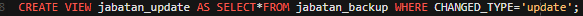
\includegraphics[width=.8\textwidth]{fifure/24.PNG}
    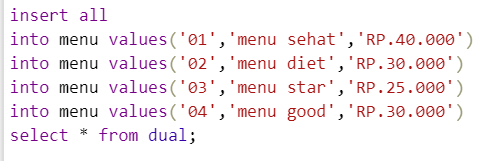
\includegraphics[width=.8\textwidth]{fifure/25.PNG}
    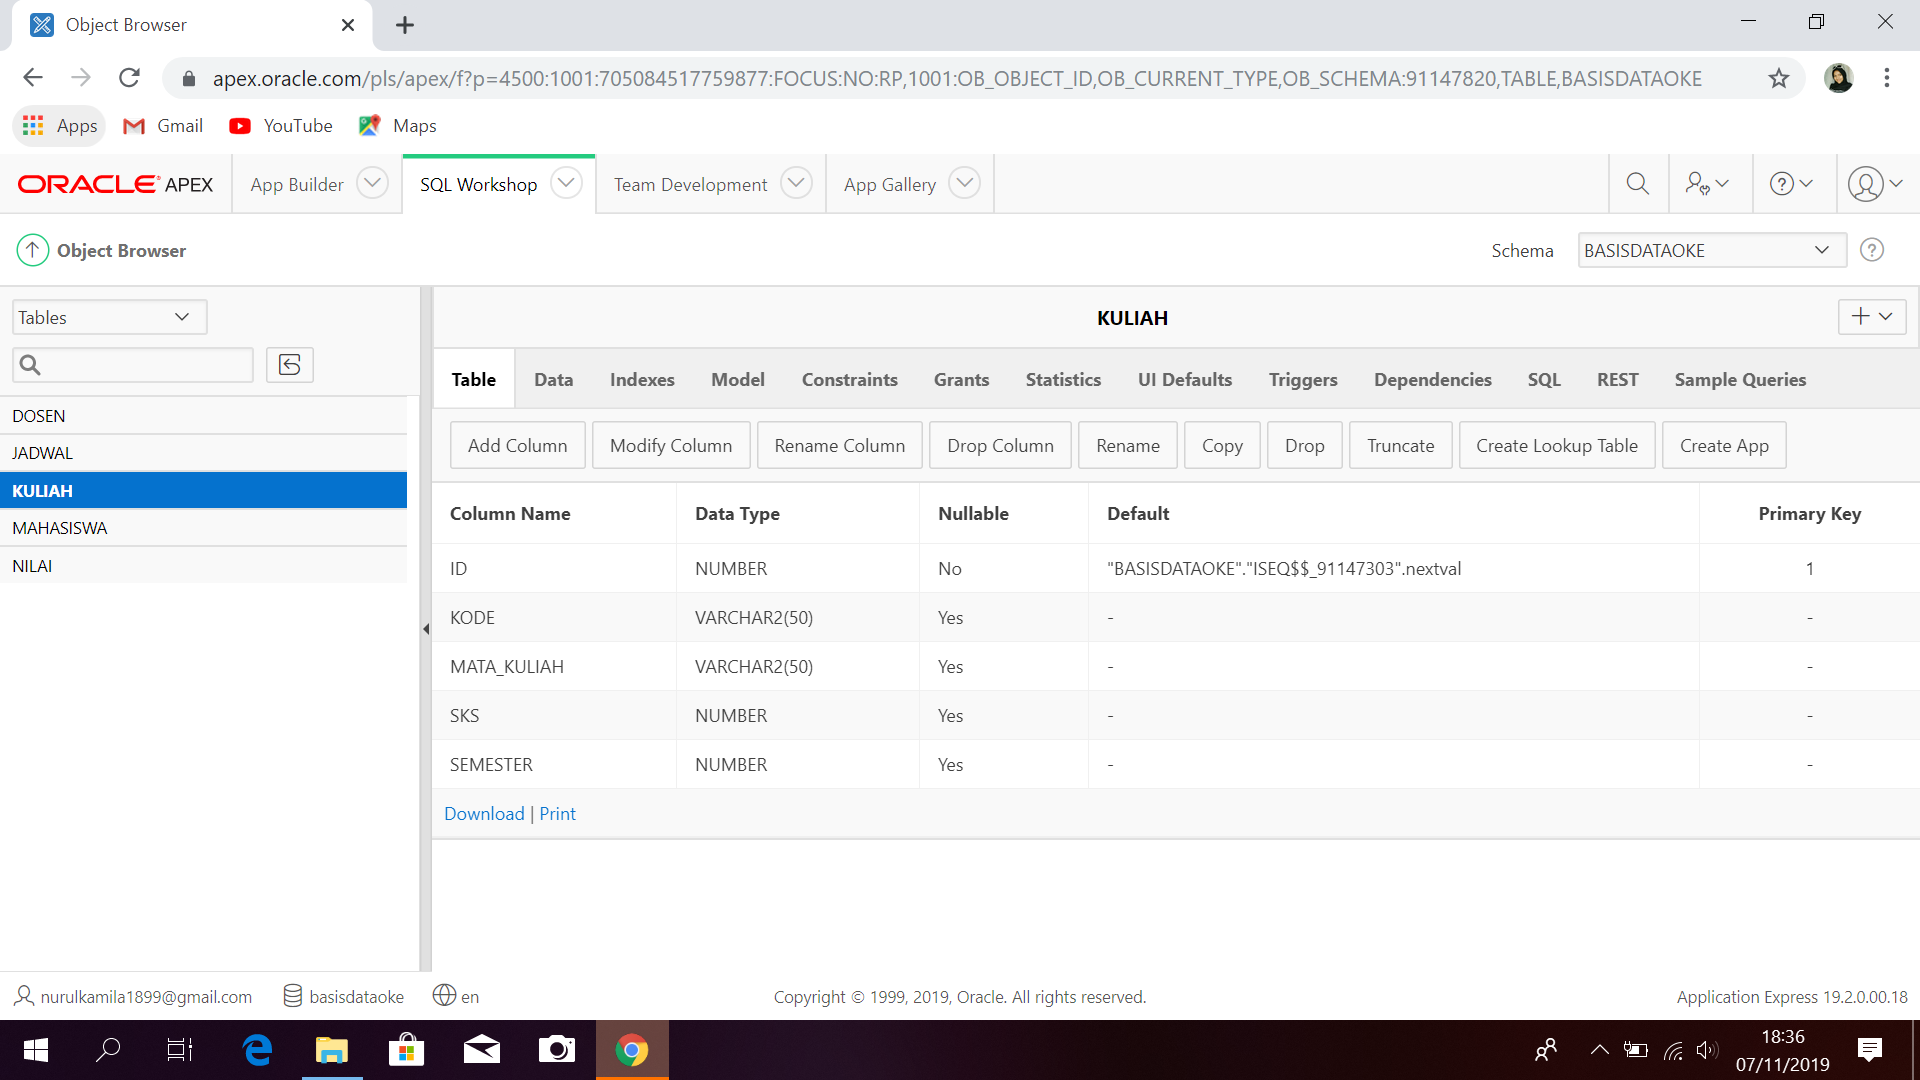
\includegraphics[width=.8\textwidth]{fifure/26.PNG}
    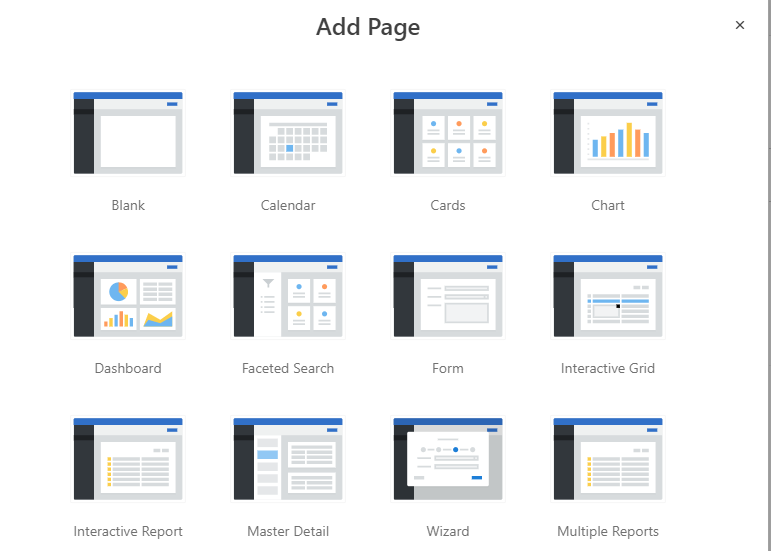
\includegraphics[width=.8\textwidth]{fifure/27.PNG}
    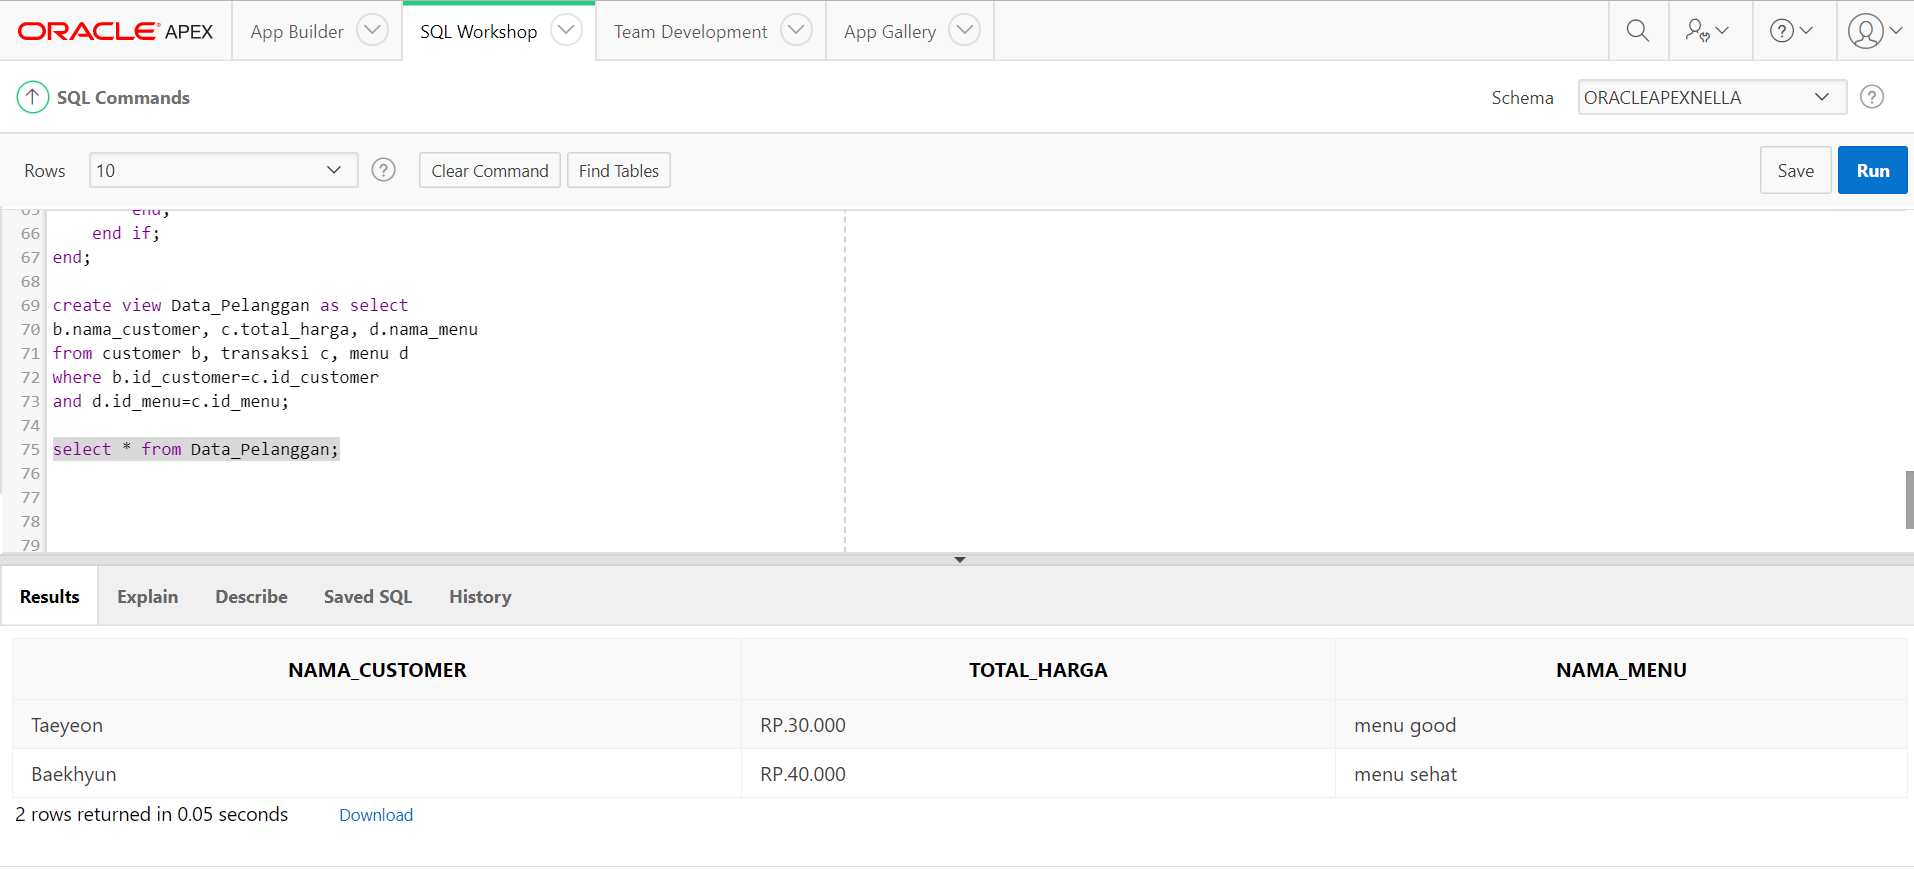
\includegraphics[width=.8\textwidth]{fifure/29.PNG}
    \end{center}
    \item setelah itu, pada pilihan constrains, setting primery key, dan foregent key sesuai tabel 
    \begin{center}
    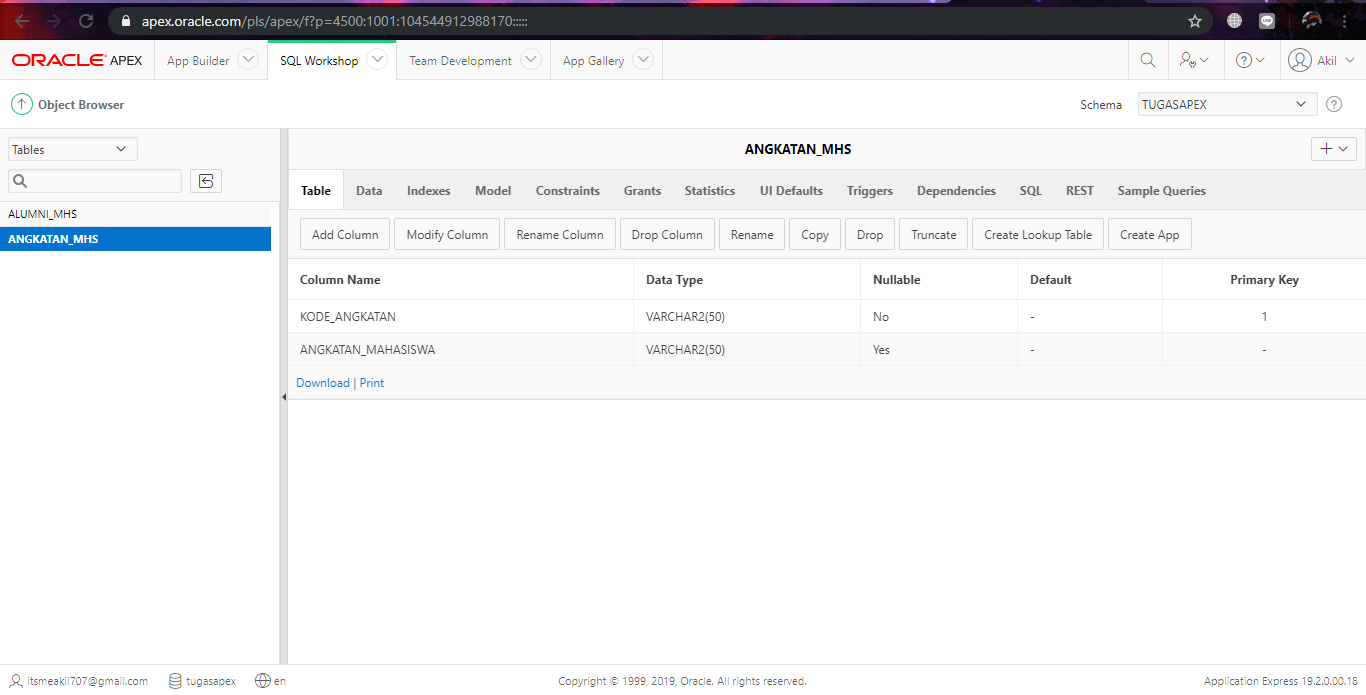
\includegraphics[width=.8\textwidth]{fifure/30.PNG}
    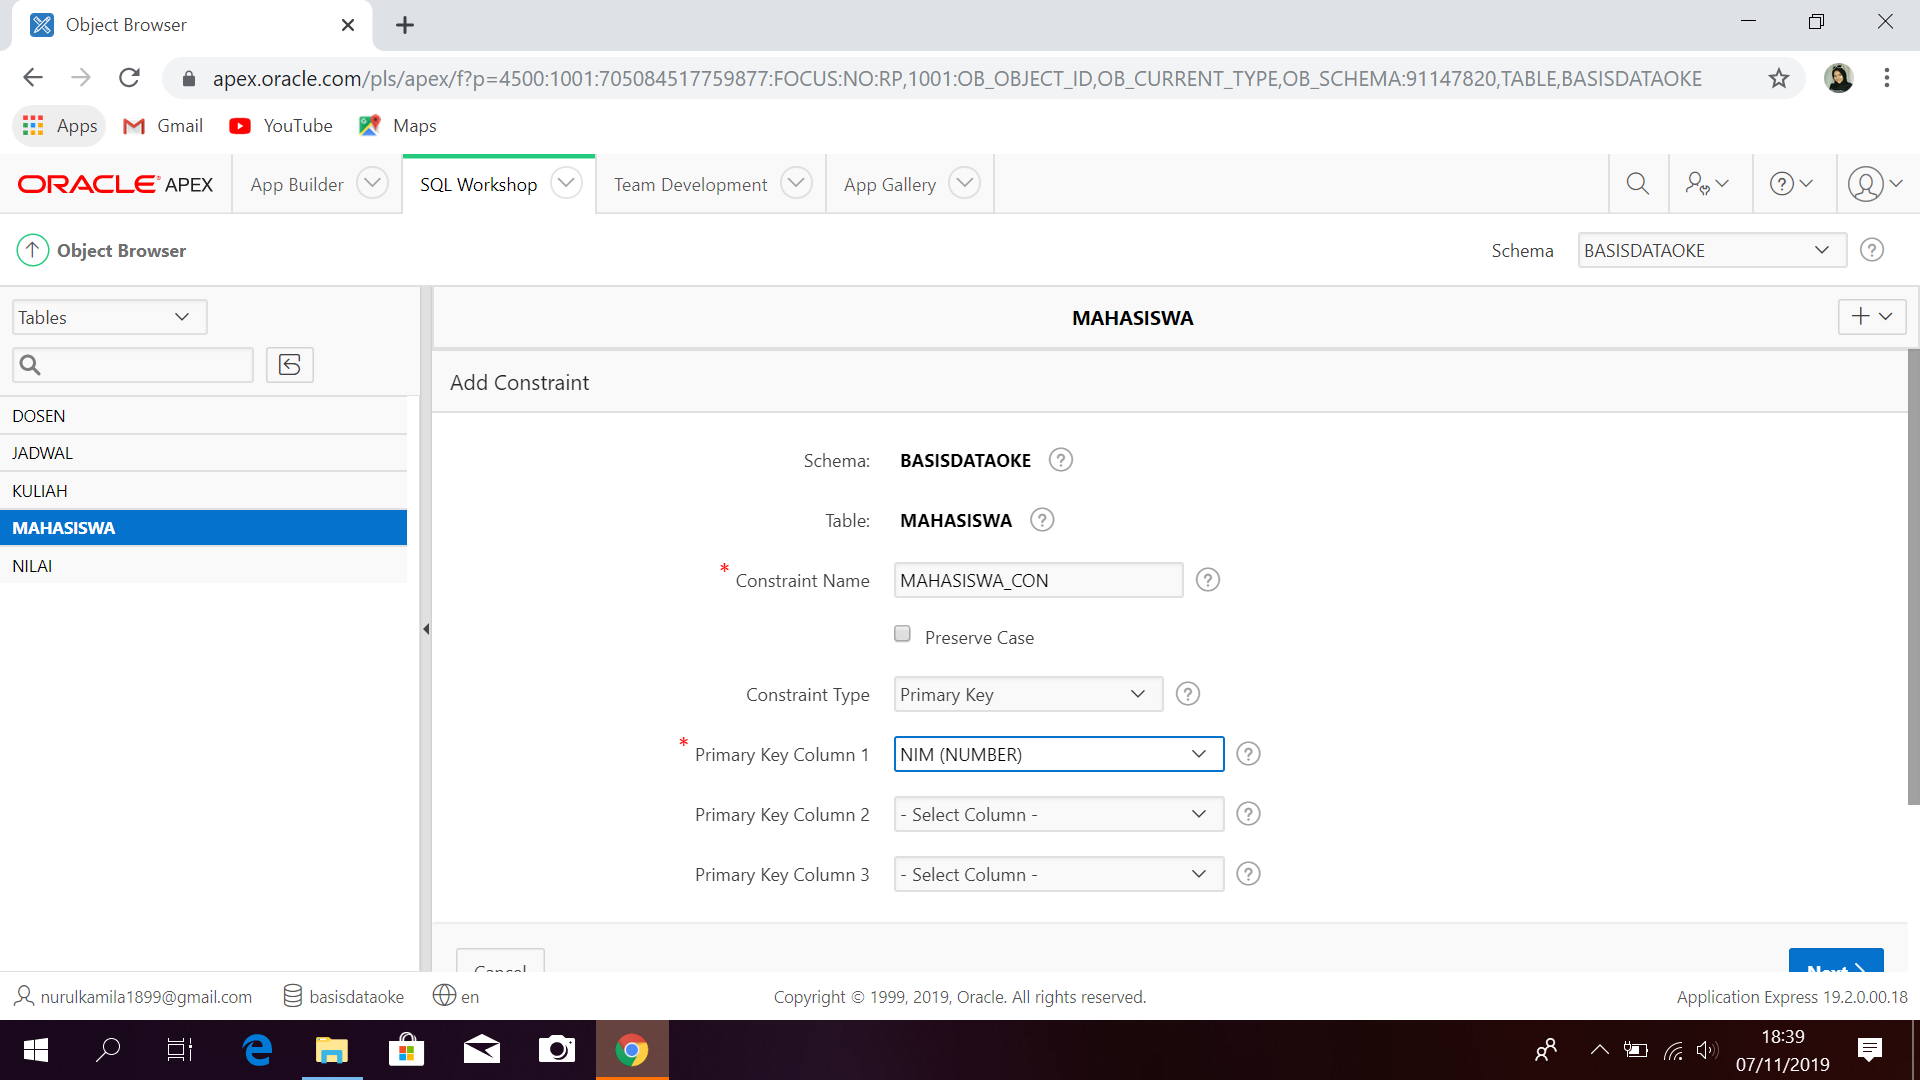
\includegraphics[width=.8\textwidth]{fifure/31.PNG}
    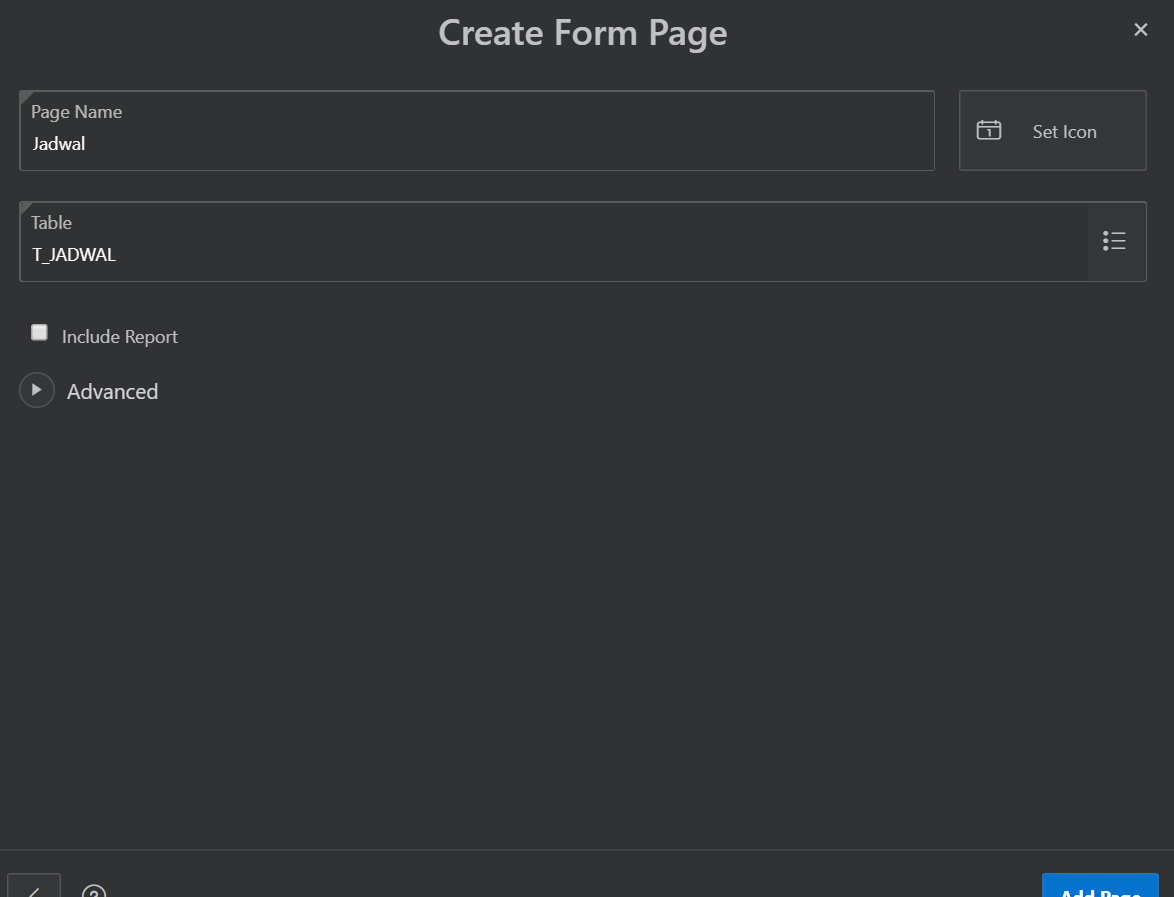
\includegraphics[width=.8\textwidth]{fifure/32.PNG}
    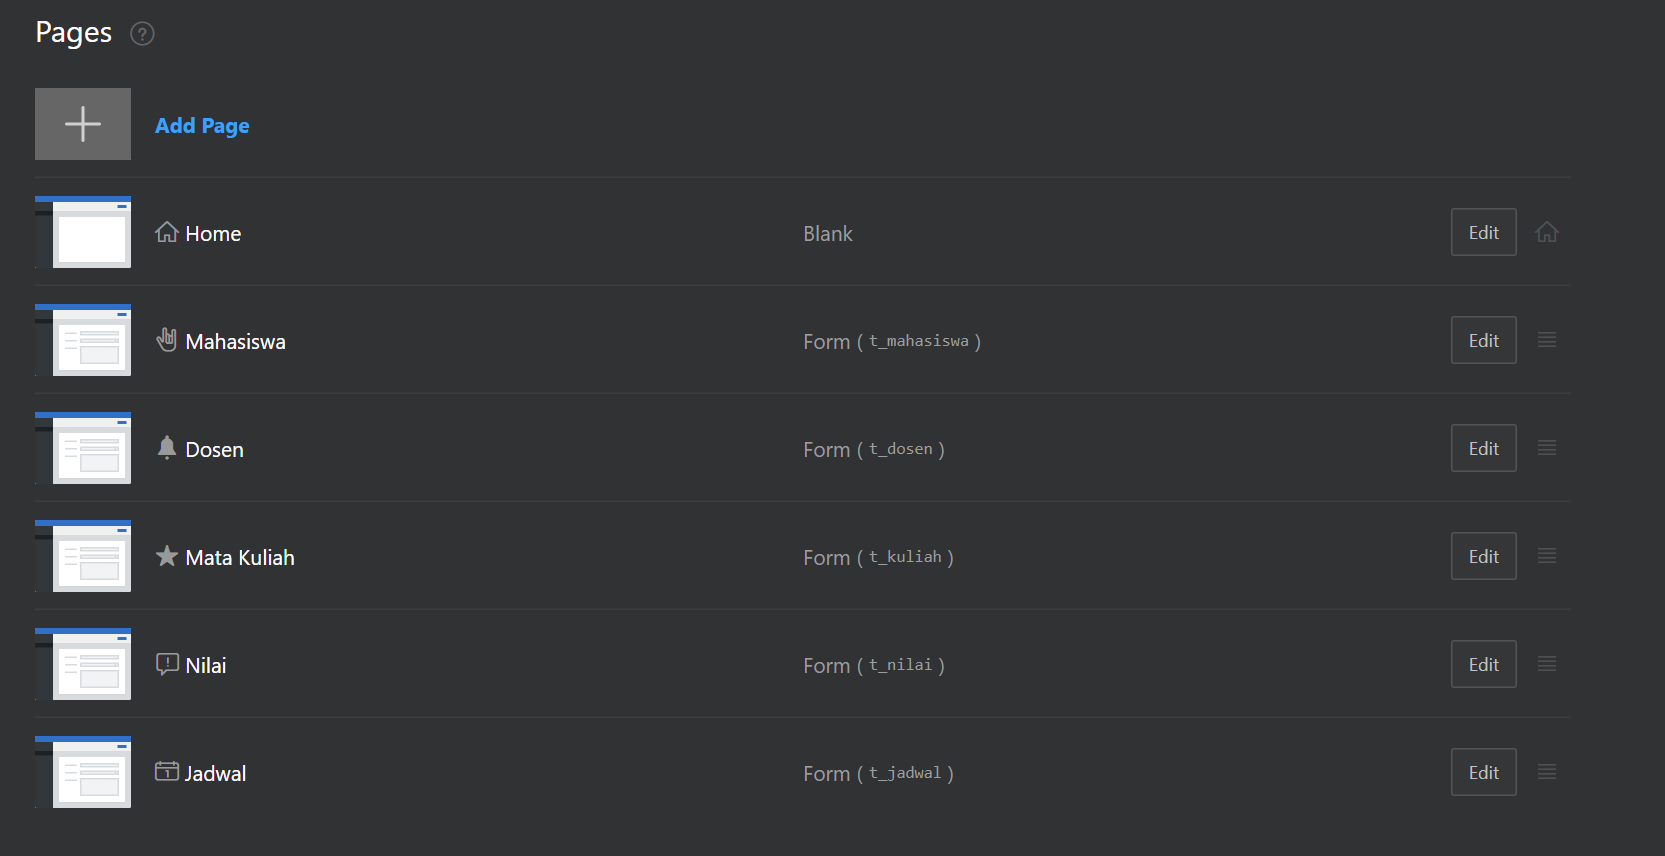
\includegraphics[width=.8\textwidth]{fifure/33.PNG}
    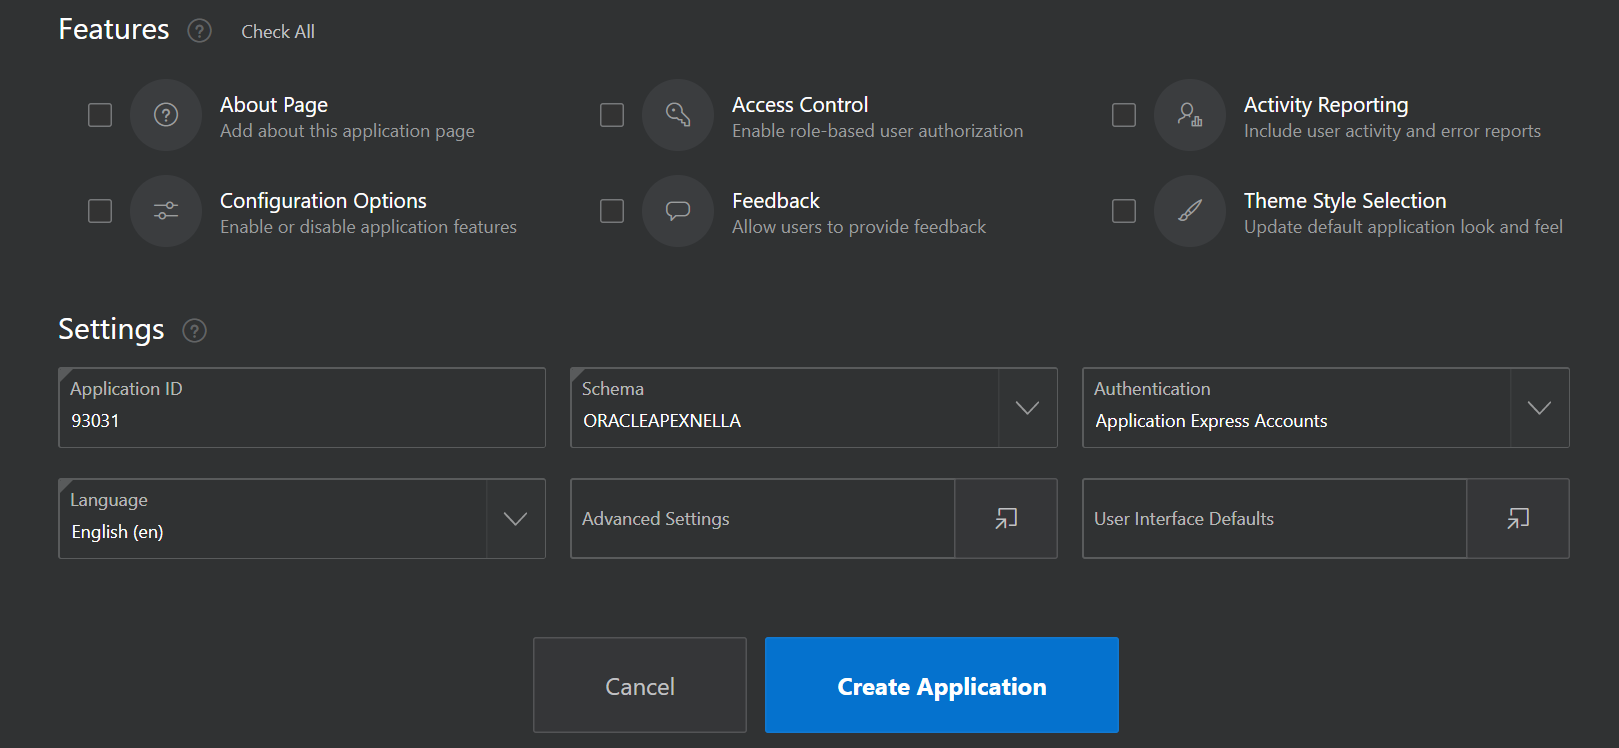
\includegraphics[width=.8\textwidth]{fifure/34.PNG}
    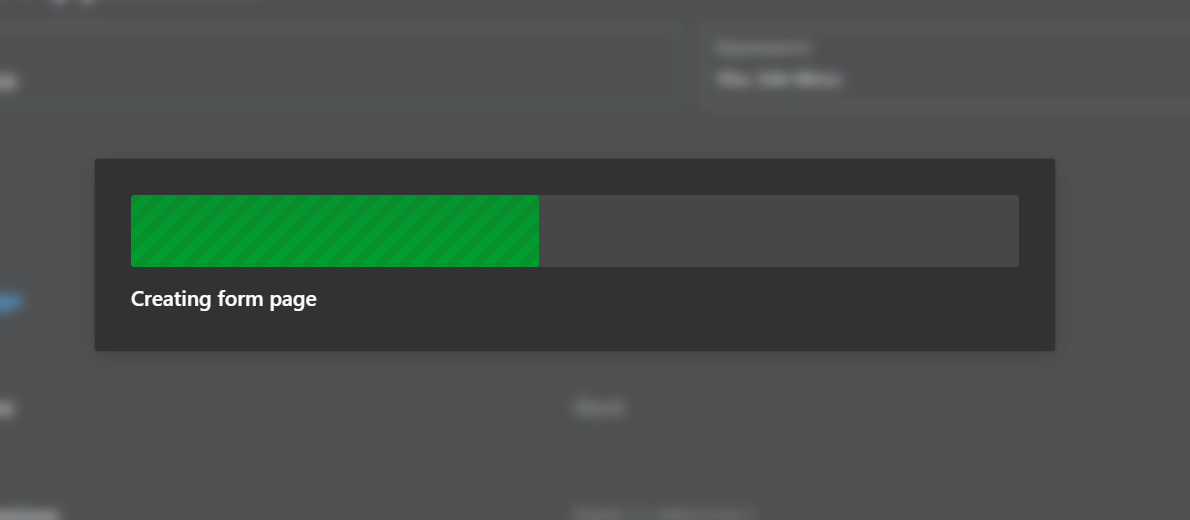
\includegraphics[width=.8\textwidth]{fifure/35.PNG}
    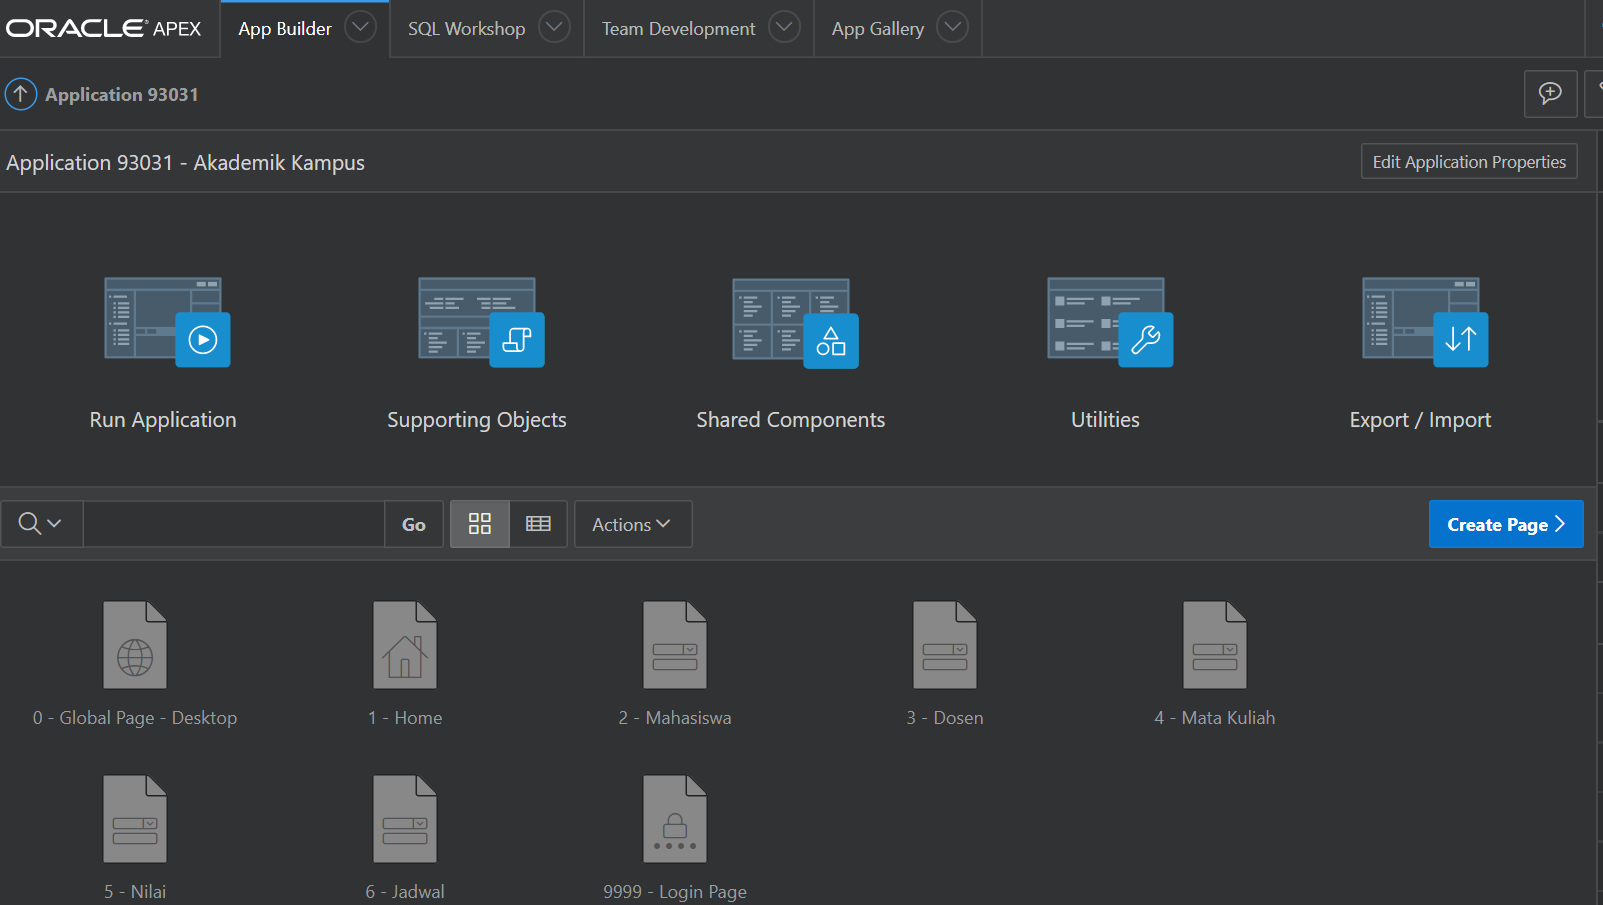
\includegraphics[width=.8\textwidth]{fifure/36.PNG}
    \end{center}
    \item Lalu, kembali ke App Builder, lalu pilih New Application
     \begin{center}
    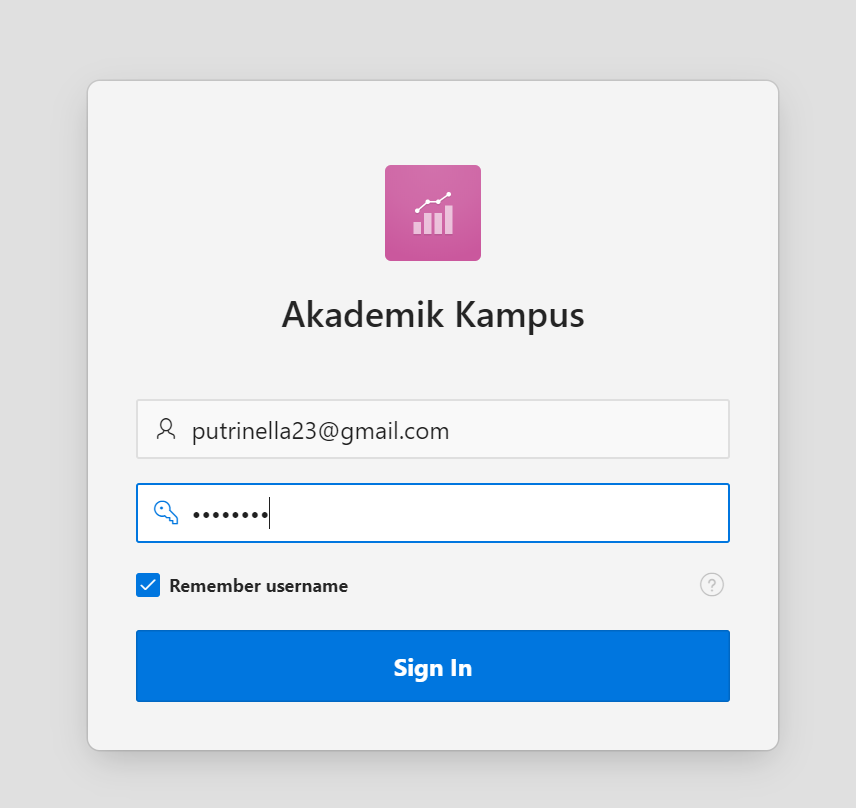
\includegraphics[width=.8\textwidth]{fifure/37.PNG}
    \end{center}
    \item Add Page , lalu pilih Interactive Report
     \begin{center}
    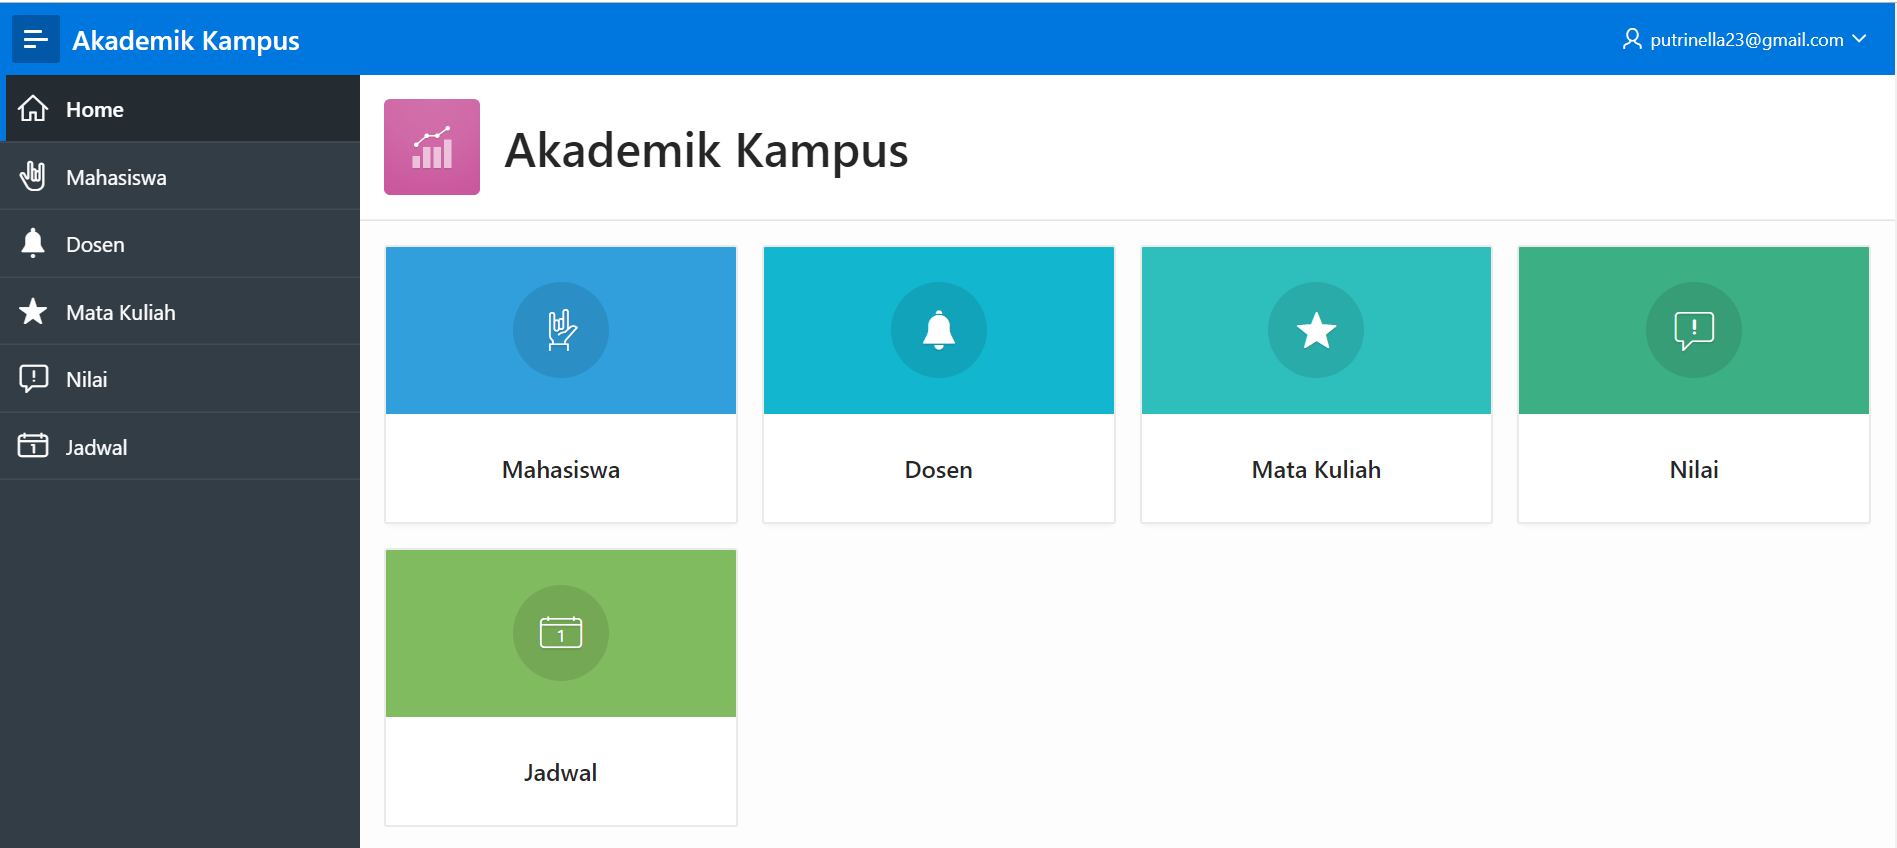
\includegraphics[width=.8\textwidth]{fifure/38.PNG}
     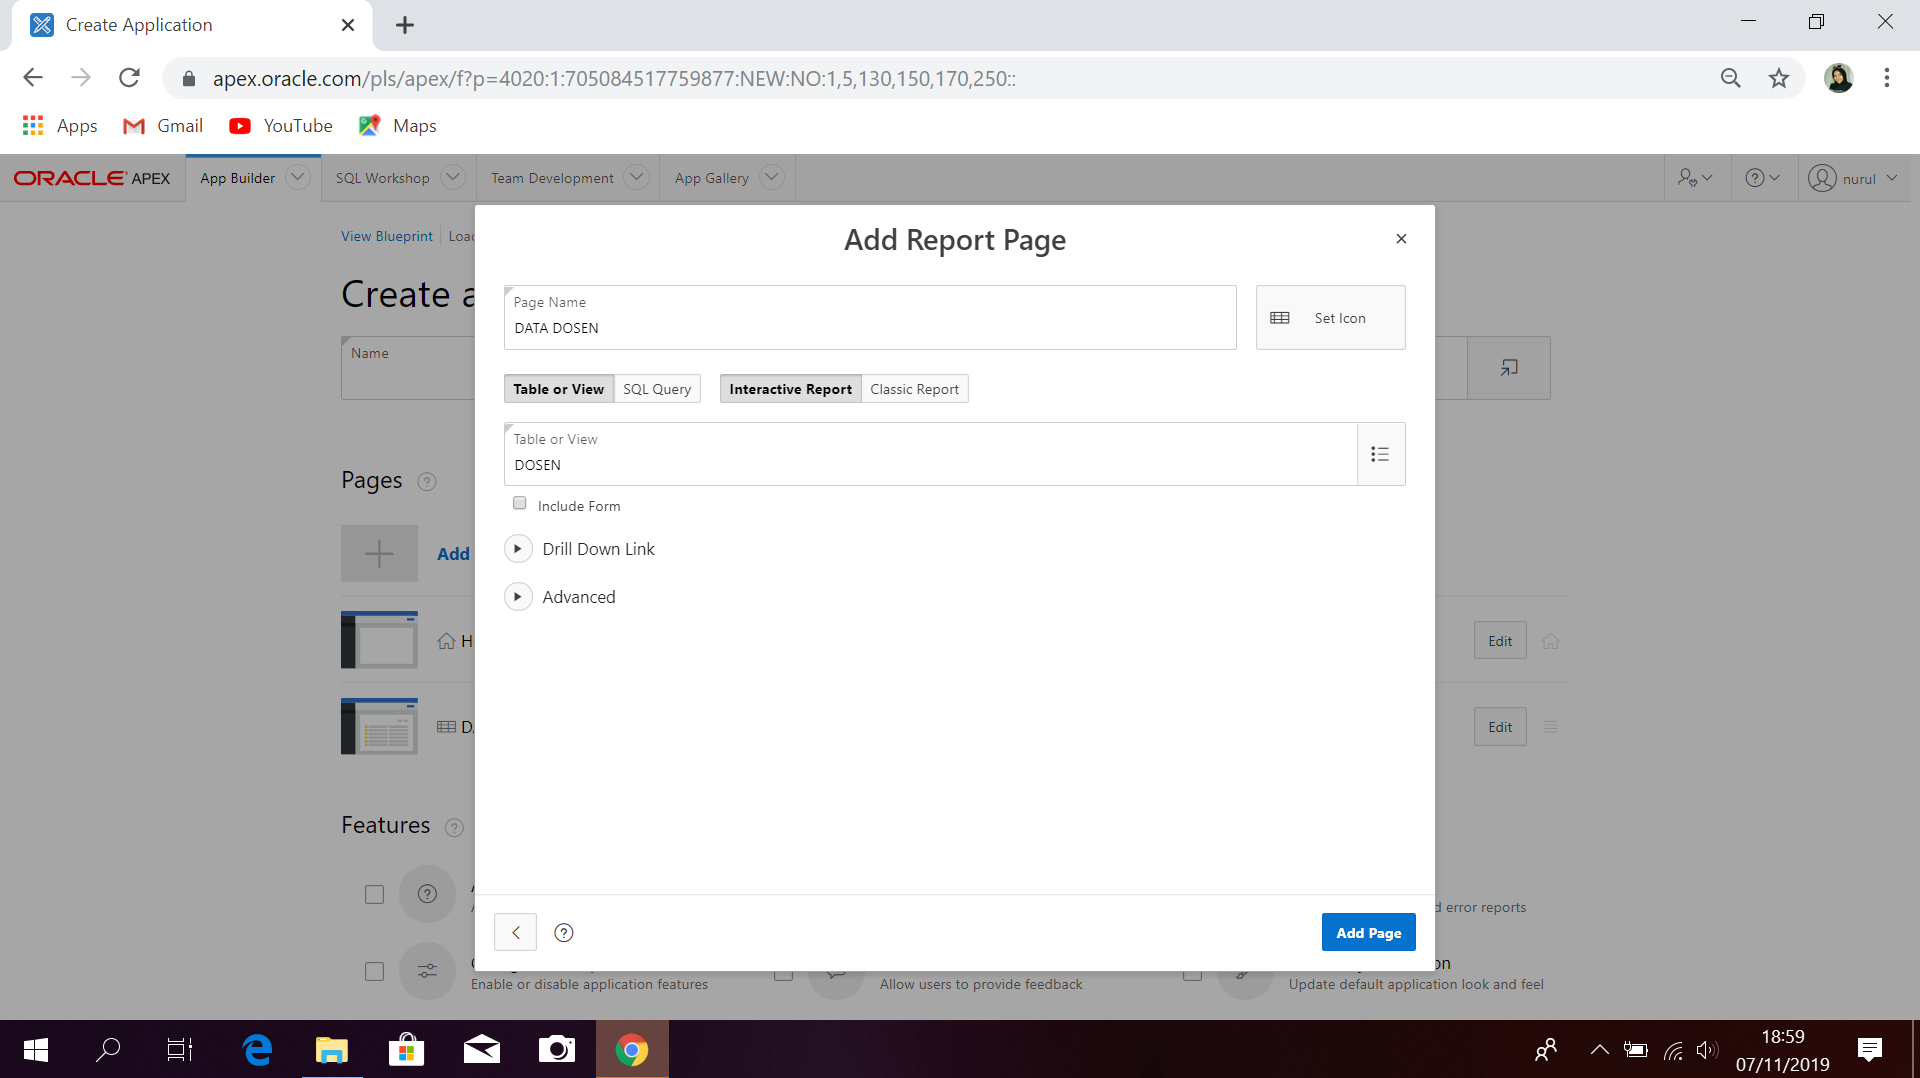
\includegraphics[width=.8\textwidth]{fifure/39.PNG}
      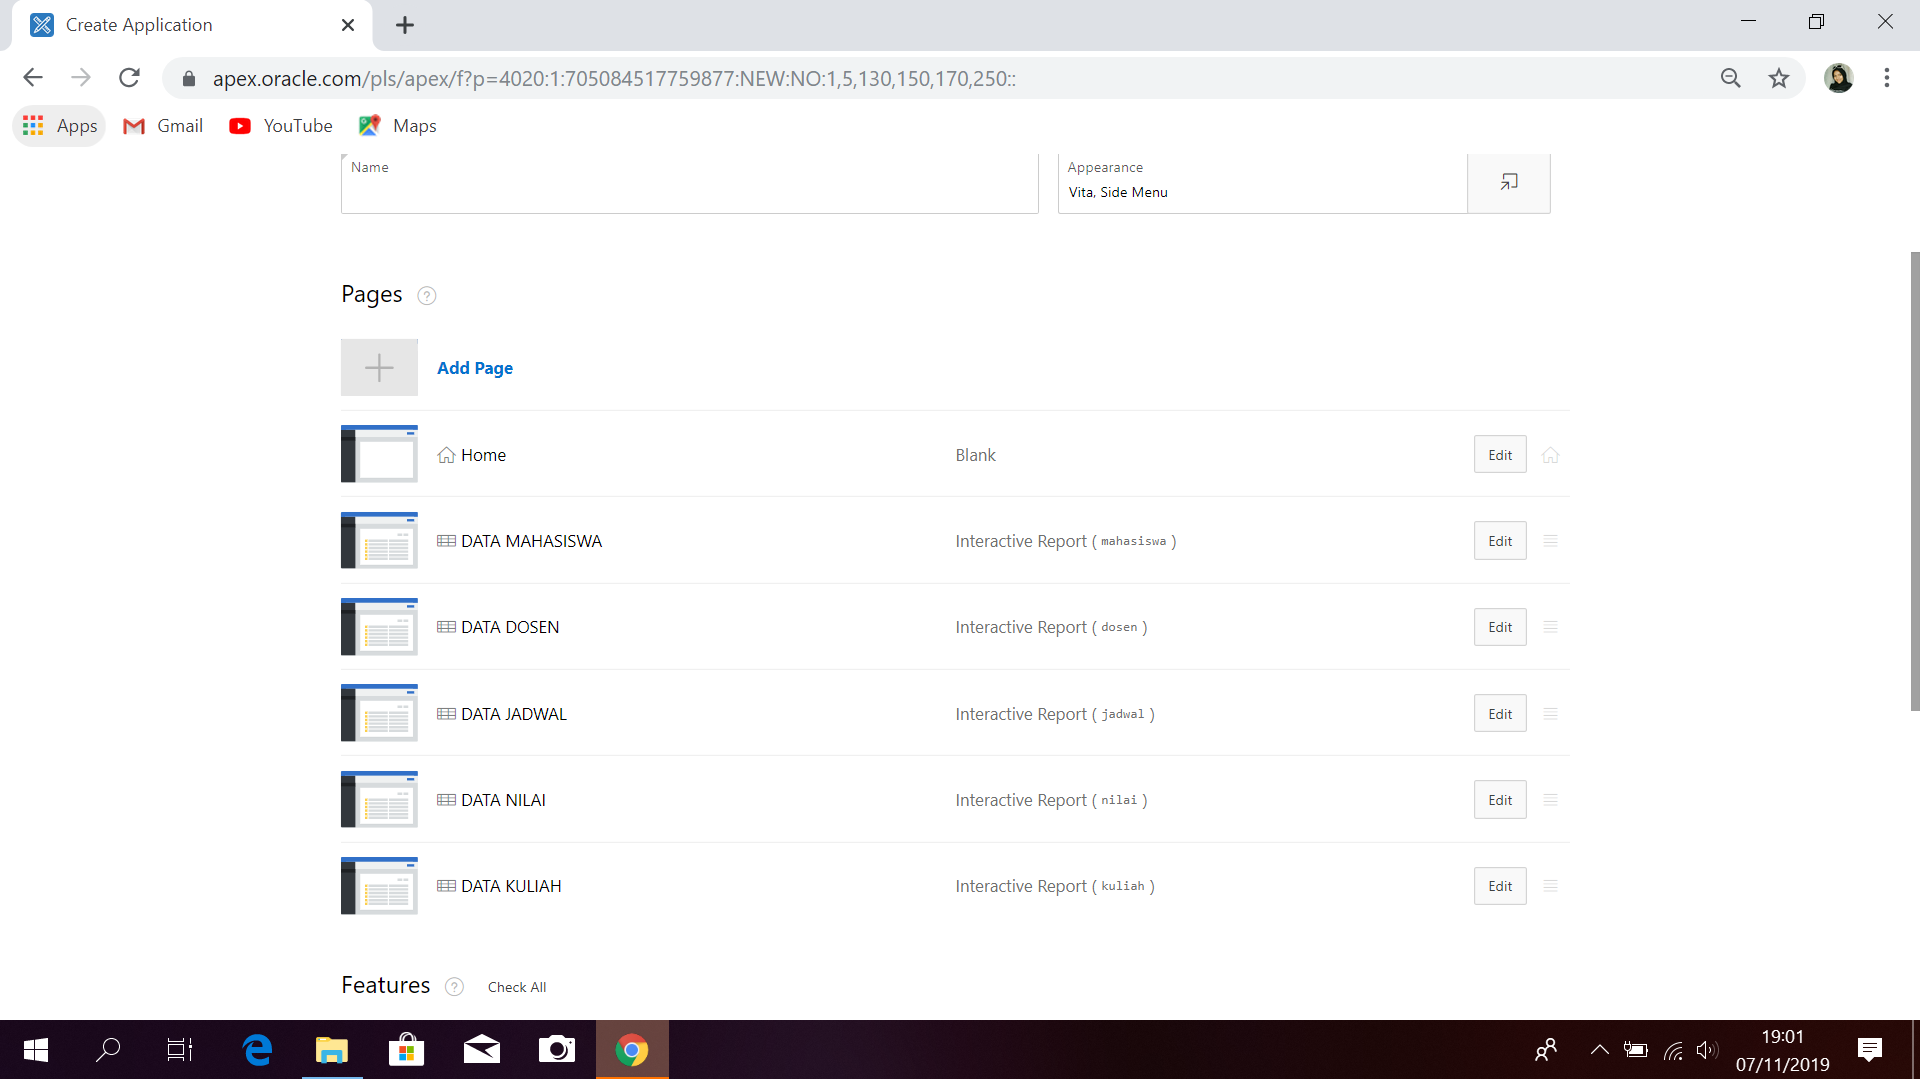
\includegraphics[width=.8\textwidth]{fifure/40.PNG}
       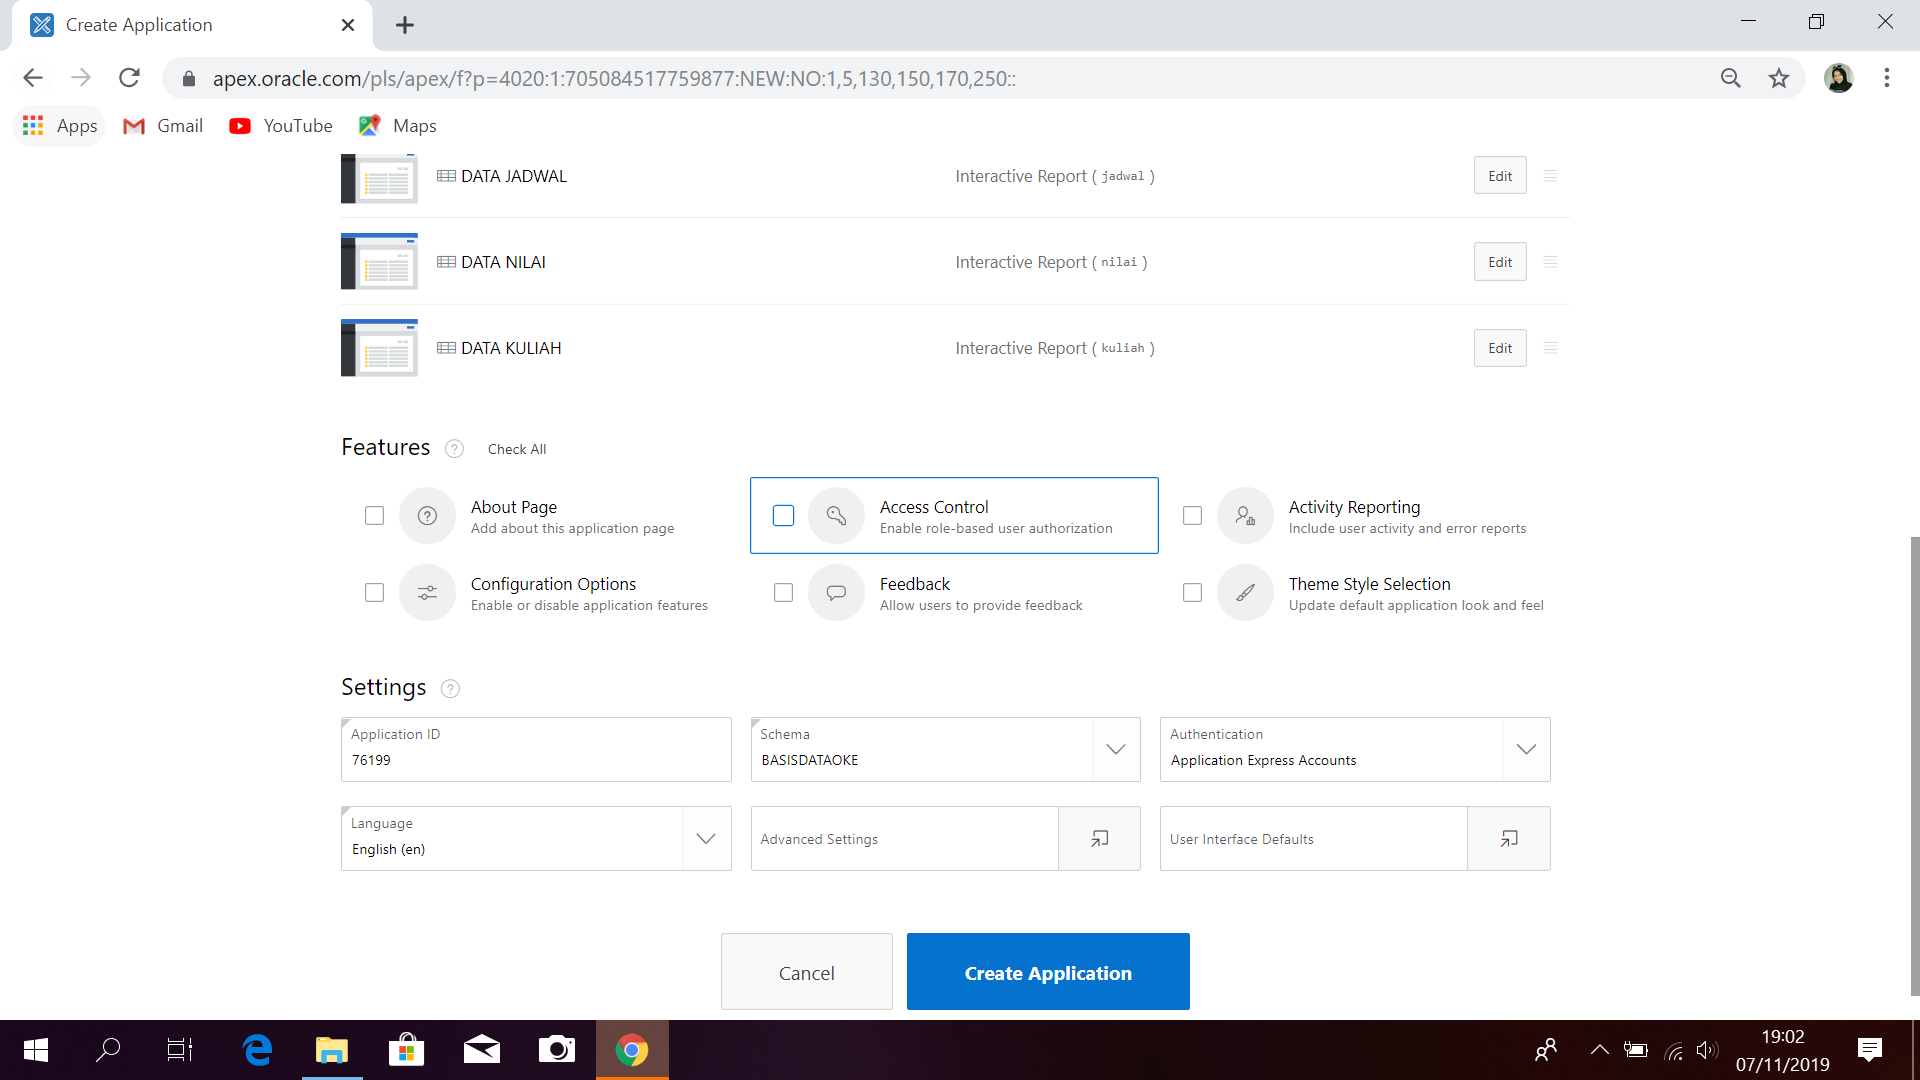
\includegraphics[width=.8\textwidth]{fifure/41.PNG}
    \end{center}
    \item jika sudah semua, Run Application
     \begin{center}
    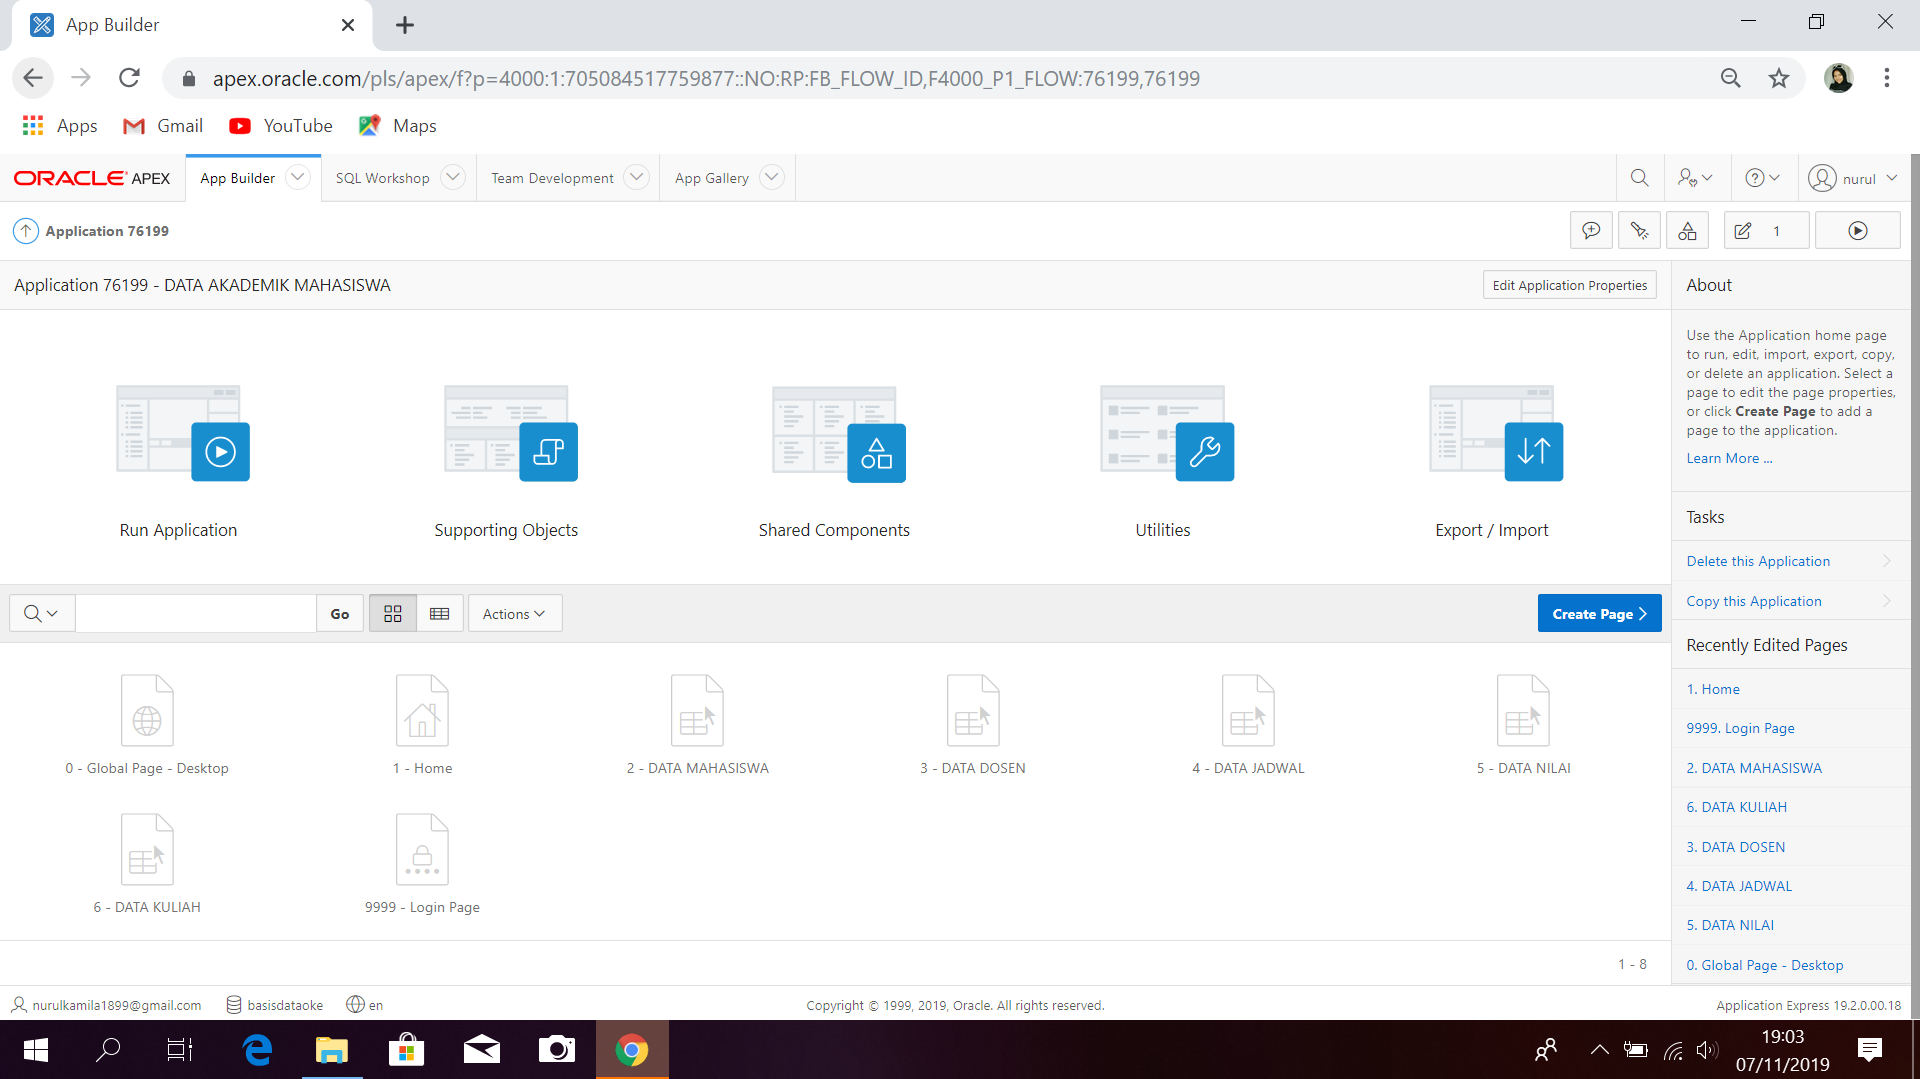
\includegraphics[width=.8\textwidth]{fifure/42.PNG}
    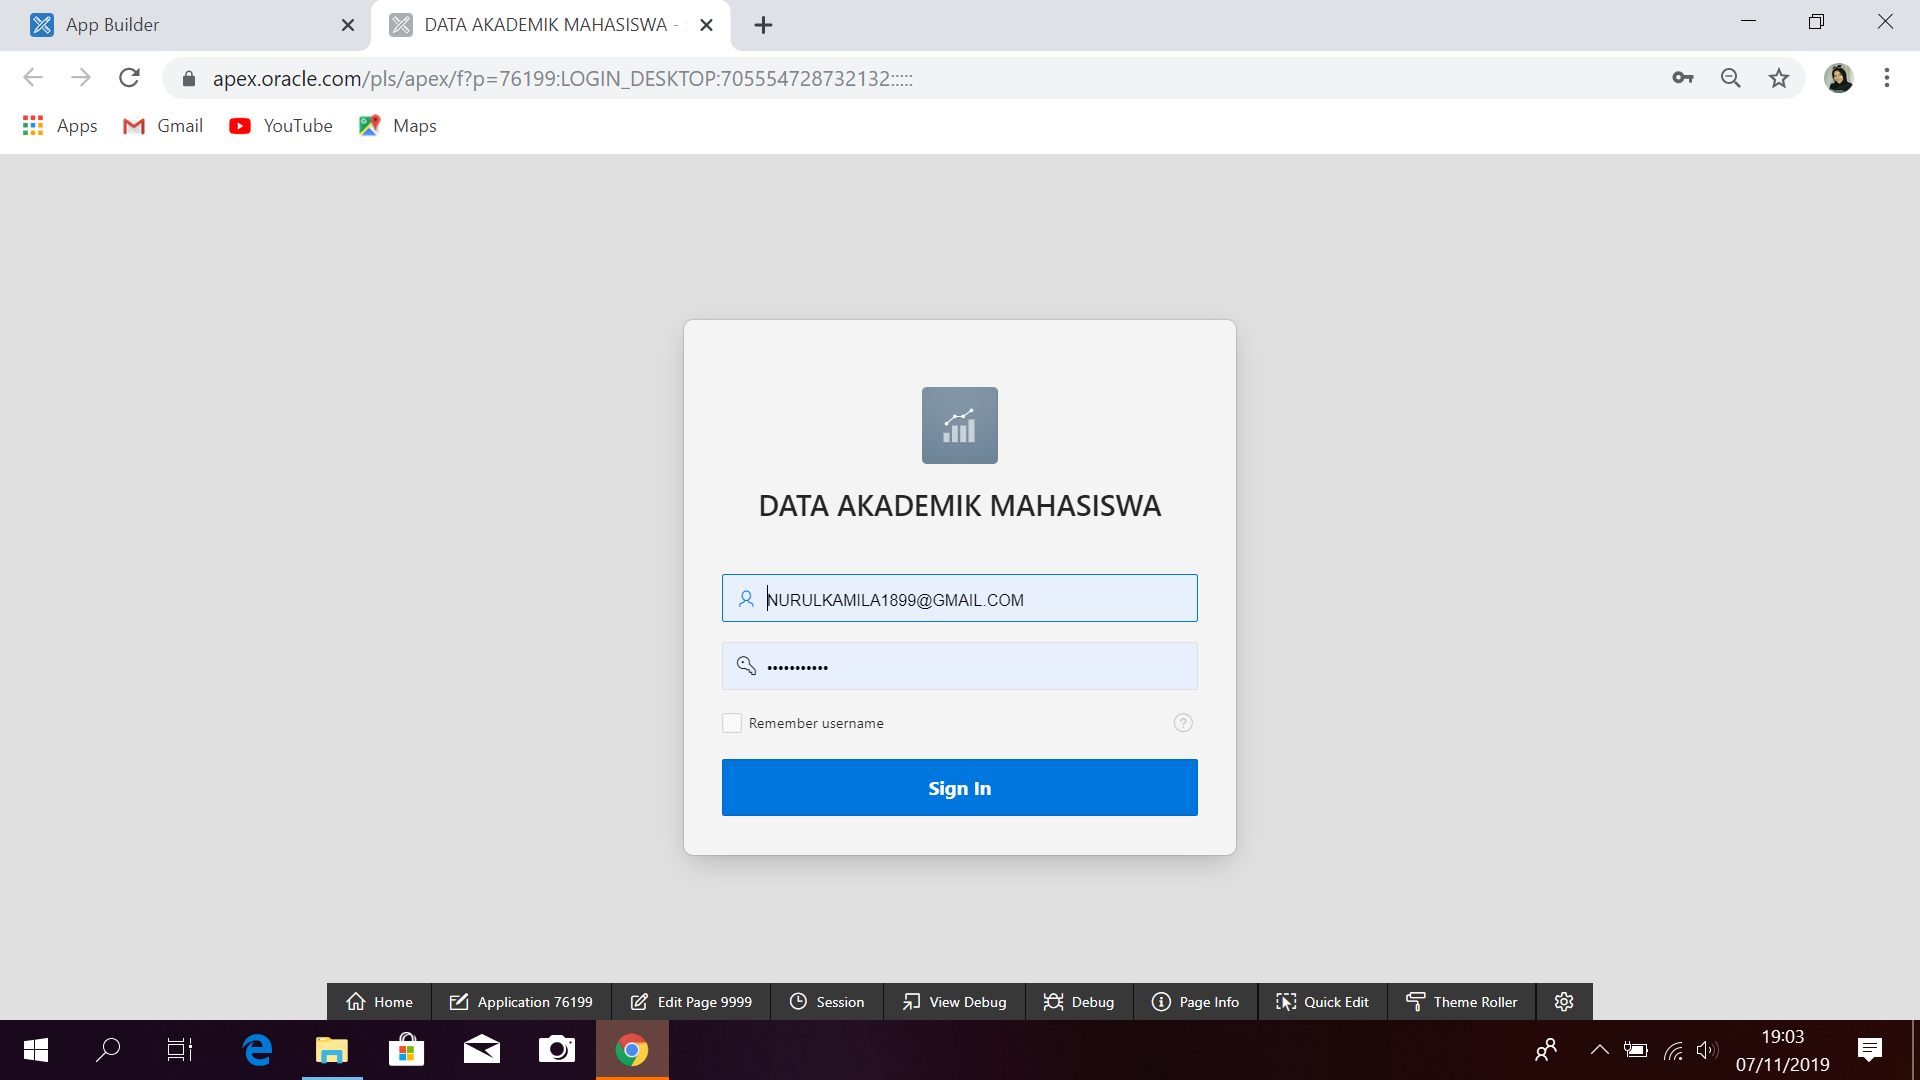
\includegraphics[width=.8\textwidth]{fifure/43.PNG}
    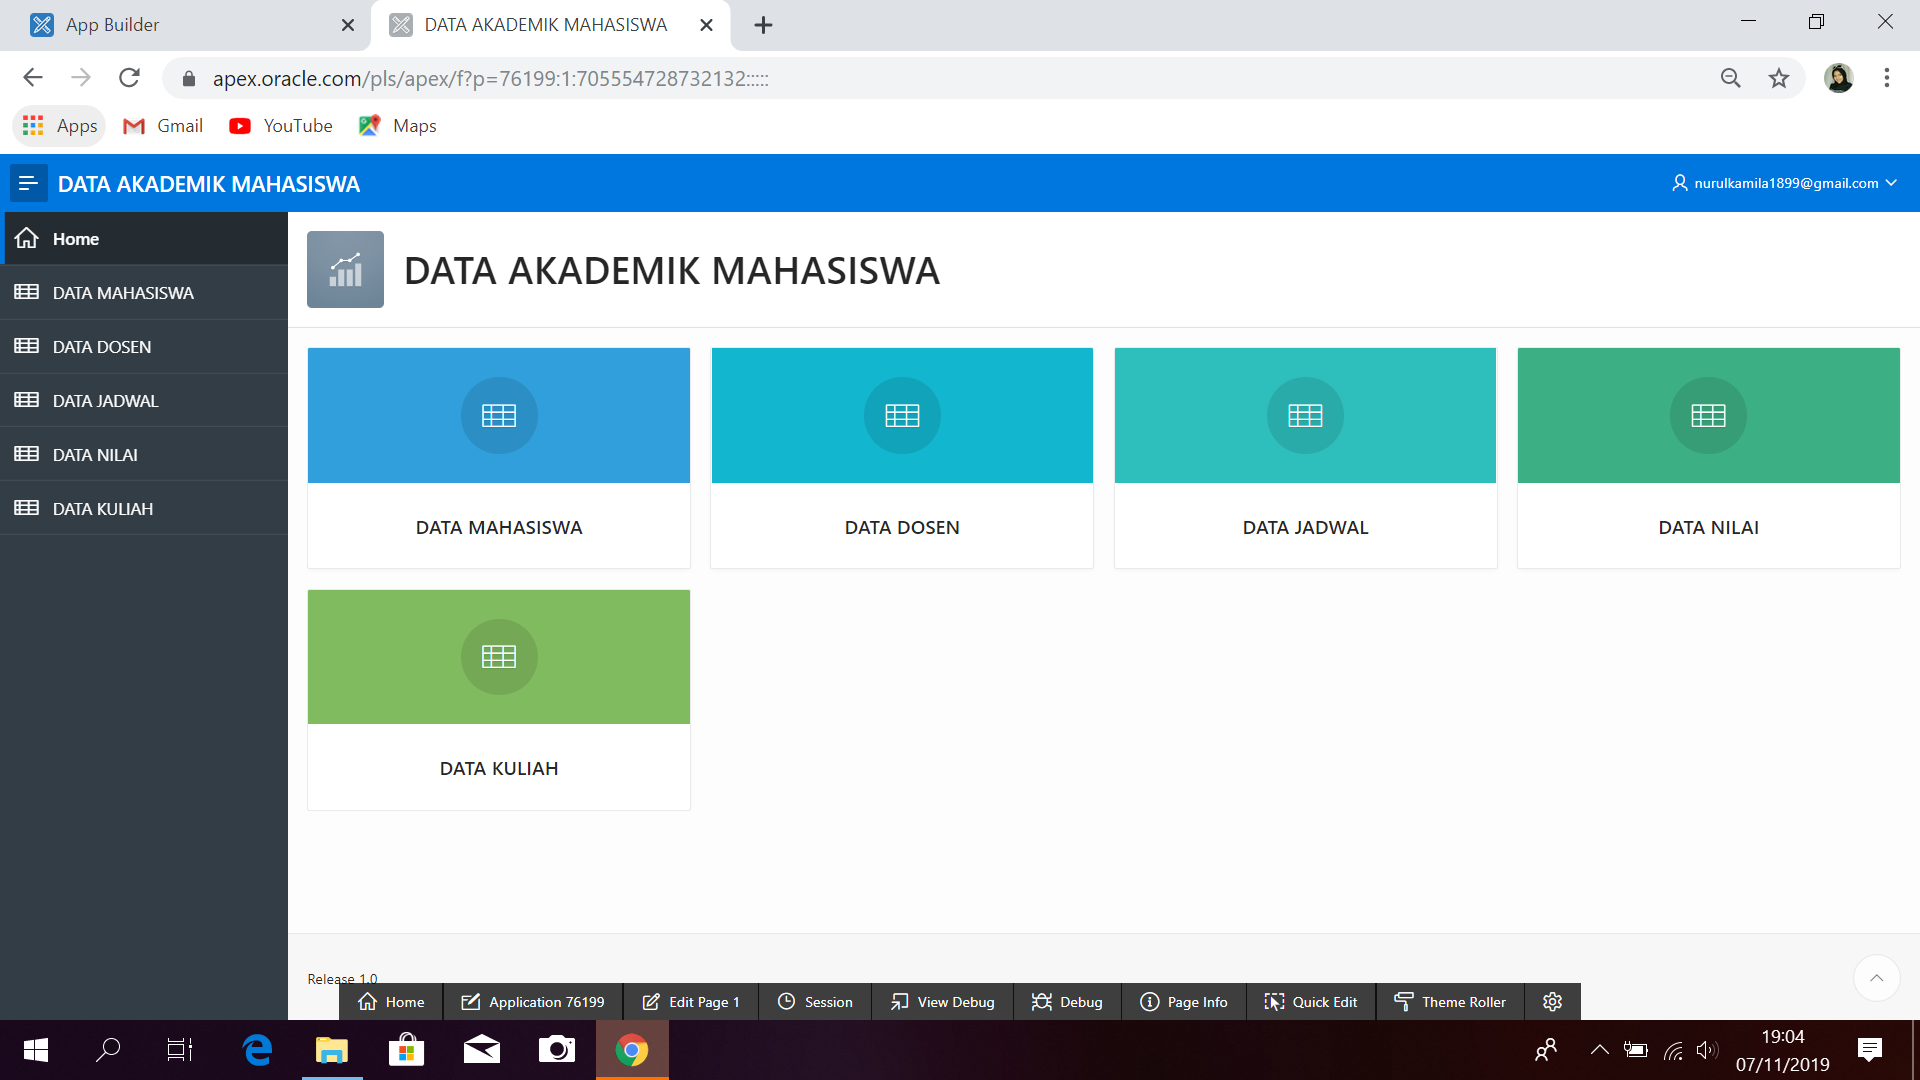
\includegraphics[width=.8\textwidth]{fifure/44.PNG}
    \end{center}
\end{enumerate}

\section{link login  https://apex.oracle.com/pls/apex/f?p=76199:LOGIN_DESKTOP:102738448248248::::: \\
Username : NURULKAMILA1899@GMAIL.COM \\
Password :twentytwo22 }

\end{document}
